\documentclass[
paper = a4,
fontsize = 12pt,
headinclude = true,
% start chapters on the right side
open = right,
% Use twosided layout? Every chapter starts on the right side, therefore sometimes blank pages are added between chapters.
twoside = false,
BCOR = 10mm,
% add lists and bibliography to table of contents
toc = listofnumbered,
toc = bibnumbered,
% enumerate chapters as x.y instead of x.y.
numbers = noendperiod
]{scrreprt}
\renewcommand{\familydefault}{\sfdefault}

%-------------------------------------------------------------------------------------------%
% PACKAGES 
\usepackage[ngerman]{babel}
\usepackage[german=quotes]{csquotes}
\usepackage{tabularx}
\usepackage[hidelinks]{hyperref}
\usepackage{amsmath} % for math
\usepackage{graphicx} % for images
\usepackage{subcaption} % for images
\usepackage{float}
\usepackage[utf8]{inputenc} 
\usepackage{booktabs}
\usepackage{longtable} % multipage tables
\usepackage[automark]{scrlayer-scrpage}
\usepackage{parskip} % turn off indents
\usepackage{listings} % code segments
\usepackage[table,xcdraw]{xcolor} % colors for listing format config
%%Java Code im Stil von Eclipse
\definecolor{javared}{rgb}{0.6,0,0} % for strings
\definecolor{javagreen}{rgb}{0.25,0.5,0.35} % comments
\definecolor{javapurple}{rgb}{0.5,0,0.35} % keywords
\definecolor{javadocblue}{rgb}{0.25,0.35,0.75} % javadoc
  
\lstdefinestyle{Java}{language=Java,
	basicstyle=\footnotesize\ttfamily,
	keywordstyle=\color{javapurple}\bfseries,
	stringstyle=\color{javared},
	commentstyle=\color{javagreen},
	morecomment=[s][\color{javadocblue}]{/**}{*/},
	numbers=left,
	numberstyle=\small\color{black},
	stepnumber=1,
	numbersep=10pt,
	tabsize=4,
	showspaces=false,
	showstringspaces=false,
	breaklines=true,
	frame=single
}


% HTML Code Style
\definecolor{htmlblue}{HTML}{2a71b8} % for tags
\definecolor{htmlpurple}{HTML}{703fa6} % for "" enclosed
\definecolor{htmlpink}{HTML}{e97bdb} % unused

\lstdefinelanguage{HTML}{
	sensitive=true,
	keywords={html, title, meta, style, head, body, h1, h2, h3, p},
	otherkeywords={<, >, /},
	morestring=[b]"
}

\lstdefinestyle{HTML}{language=HTML,
	basicstyle=\footnotesize\ttfamily,
	keywordstyle=\color{htmlblue}\bfseries,
	stringstyle=\color{htmlpurple},
	numbers=left,
	numberstyle=\small\color{black},
	stepnumber=1,
	numbersep=10pt,
	tabsize=4,
	showspaces=false,
	showstringspaces=false,
	breaklines=true,
	frame=single
}
	
	

%%Python Code im Stil von Eclipse
\definecolor{red}{rgb}{1,0,0} % keywords

\lstdefinestyle{Python}{language=Python,
	basicstyle=\ttfamily,
	keywordstyle=\color{javapurple}\bfseries,
	stringstyle=\color{javared},
	commentstyle=\color{javagreen},
	morecomment=[s][\color{javadocblue}]{/**}{*/},
	numbers=left,
	numberstyle=\tiny\color{black},
	stepnumber=1,
	numbersep=10pt,
	tabsize=4,
	showspaces=false,
	showstringspaces=false
}
 % code listing config
\lstset{
	  basicstyle=\footnotesize\ttfamily
}
\renewcommand{\lstlistingname}{Quellcode} % change 'Listing' to 'Quellcode'
\renewcommand{\lstlistlistingname}{Quellcodeverzeichnis}

\usepackage{pdfpages} % include excel pdf

\usepackage{tocloft}
\setlength\cftbeforechapskip{5pt}
\setlength\cftbeforepartskip{15pt}

\usepackage[export]{adjustbox}

\usepackage{multirow}


%-------------------------------------------------------------------------------------------%
% BIBLIOGRAPHY
\usepackage[backend=bibtex,style=verbose-trad2]{biblatex}
\bibliography{bibliography/citations_gwercher}
\bibliography{bibliography/citations_egger}

%-------------------------------------------------------------------------------------------%
% VARIABLES
\newcommand{\mytitle}{NWES-SESD} 
\newcommand{\mysubtitle}{-}
\newcommand{\myschool}{Höhere Technische Bundeslehr- und Versuchsanstalt Anichstraße} 
\newcommand{\myinstitute}{Abteilung für Wirtschaftsingenieure/Betriebsinformatik} 
\newcommand{\mysubmissionyear}{2024}
\newcommand{\mysubmissionmonth}{-}
\newcommand{\myauthor}{Gwercher}
\newcommand{\mysupervisor}{-}

\newcommand{\mysubject}{SUBJECT}  %% also used for PDF metadata (hyperref)
\newcommand{\mykeywords}{KEYWORDS}  %% also used for PDF metadata (hyperref)

%-------------------------------------------------------------------------------------------%
% HEADERS & FOOTERS
\newcommand{\normalHeaderFooter}{%
	\ihead*{
\includegraphics[width=0.45\linewidth]{figures/anich_logo.png}}
	\chead*{}
	\ohead*{
\includegraphics[width=0.2\linewidth]{figures/htl_logo.png}}
	
	\ifoot*{\myauthor}
	\cfoot*{}
	\ofoot*{\thepage}
}

\newcommand{\normalFooter}{%
	\ifoot{\myauthor}
	\cfoot{}
	\ofoot{\thepage}
}

\newcommand{\noHeader}{%
	\ihead{}
	\chead{}
	\ohead{}
}

\newcommand{\noFooter}{%
	\ifoot{}
	\cfoot{}
	\ofoot{}
}


\clearpairofpagestyles
\normalHeaderFooter	
\pagestyle{scrheadings}

%-------------------------------------------------------------------------------------------%


\begin{document}
%-------------------------------------------------------------------------------------------%
% PREAMBLE PART
	\noFooter
	\pagenumbering{gobble}
		\begin{center}
	\vspace*{1cm}
	{\huge Matura}\\
	\bigskip
	{\LARGE \mytitle} \\
	\smallskip
	{\large \myschool} \\
	\bigskip
	\hrule
	\bigskip
	{\large \myinstitute} \\
	
	\bigskip
	Ausgeführt im Schuljahr 2024 von: \\
	\myauthor \\
	\bigskip


\end{center}
	
	\normalFooter 
	\pagenumbering{roman} \setcounter{page}{1}
	
	\tableofcontents
	\newpage
%-------------------------------------------------------------------------------------------%
% MAIN PART
	\pagenumbering{arabic} 
	\setcounter{page}{1}
	\part{4BHWII}
	\chapter{IPv4 (Internet Protocol Version 4)}
Eine IPv4-Adresse ist eine 32-Bit Zahl. Es gibt also $2^{32}$ $\approx$ 4,3 Milliarden IPv4-Adressen.

\begin{table}[H]
	\begin{tabular}{c|c|c|c}
		 \multicolumn{4}{l}{\textbf{Bsp:}} \\
		11000000 & 10101000 & 00001010 & 00001010 \\
		192 & 168 & 10 & 10 \\
		 \multicolumn{4}{l}{$\rightarrow$ 192.168.10.10} \\
	\end{tabular}
\end{table}
\subsection*{Schreibweise:}
Die IPv4-Adresse wird in Dotted Decimal Notation geschrieben. Die IP-Adresse wird in 8-Bit Blöcke (Oktetten) geteilt, dezimal übersetzt und durch Punkte getrennt.

\subsection*{Verwendung}
Jedes Gerät soll durch eine Adresse (IP-Adresse) eindeutig identifiziert werden. Zusätzlich sollten auch Gruppen (Netze) von Computern erstellt werden (mit Subnetzmasken). Ein Gerät mit IP-Adresse nennt man Host.

\subsection*{Subnetmask}
Ist eine 32-Bit Zahl, die in Dotted Deicmal Notation beschrieben wird. Es kommen zuerst alles Einsen und nach der ersten Null nur noch Nullen. 

\subsubsection*{Typische Subnetmasken}
\begin{table}[H]
	\begin{tabular}{c|c|c}
%		\multicolumn{3}{l}{\textbf{Typische Subnetmasken:}} \\
		& Präfix & Hosts \\
		\hline
		255.0.0.0 & 8 & $2^{24}$ - 2 = 16.777.214 \\
		\hline
		255.255.0.0 & 16 & $2^{16}$ - 2 = 65.534 \\
		\hline
		255.255.255.0 & 24 & $2^{8}$ - 2 = 254
	\end{tabular}
\end{table}
\begin{table}[H]
	\begin{tabular}{cc|cc}
		\multicolumn{4}{l}{\textbf{Bsp:}} \\
		\multicolumn{2}{c}{Telefonnummer} & \multicolumn{2}{c}{IP-Adresse} \\
		+43 664 & 123456 & 172.16. & 20.25 \\
		Netz & einzigartig & 255.255. & 0.0 \\
		 & & Netzteil & Hostteil
	\end{tabular}
\end{table}
Die Subnetzmaske trennt die IP-Adresse in Netzteil und Hostteil. IP-Adresse und Subnetzmaske gehören immer zusammen.

\begin{enumerate}
	\item 2 IP-Adressen im gleichen Netz \\
	10.10.226.120 / 24 \\
	10.10.226.80 / 24 \\
	\item 2 IP-Adressen nicht im gleichen Netz \\
	11.40.30.124 / 24 \\
	14.8.50.100 / 24 \\
	\item Anzahl der Hosts \\
	$2^{8} - 2$ \\
	10.10.226.0 (Netzadresse), 10.10.226.255 (Broadcastadresse)
\end{enumerate}

192.168.20.100 / 8 \\
Netz:  192.0.0.0 \\
Broad: 192.255.255.255

\chapter{Netzwerke im Alltag und Grundbegriffe}
\subsection*{Netzwerk Komponenten}
\begin{itemize}
	\item Endgeräte (PC, Handy, Uhr, TV, Server,...)
	\item Intermediary Devices (Router, Repeater, Switch, Hub, Access Point)
	\item Übertragungsmedien (Drahtlos, Kupfer, Glasfaser)
\end{itemize}

\subsection*{Host-Aufgaben}
\begin{itemize}
	\item Client-Server-Modell
	\item Peer-to-Peer Modell
	\item[] \begin{tabbing}
		+ Komplexität ~~~~~~~~~~~~~~~~~~ \= - Security\\
		+ Leichter zum Aufsetzen ~~~~ \= - Erweiterbarkeit\\
	\end{tabbing}
\end{itemize}

\subsection*{Netzwerk Dokumentation}
\begin{itemize}
	\item Physische Topologie (Räume, ...)
	\item Logische Topologie (Netze, ...)
\end{itemize}

\subsection*{Netzwerke nach Größe}
\begin{itemize}
	\item SOHO ... small office home office
	\item LAN ... local area network
	\item MAN ... metropolitan area network
	\item WAN ... wide area network
	\item Internet
\end{itemize}

\subsection*{Netzwerke nach Funktion}
\begin{itemize}
	\item SAN ... storage area network
	\item Intranet, Extranet
\end{itemize}

\subsection*{Internetzugang}
\begin{itemize}
	\item Kabel (Glasfaser)
	\item DSL / Dial Up
	\item Mobilfunknetz
	\item Satellit
\end{itemize}

\subsection*{Trends}
\begin{itemize}
	\item Video / Streaming
	\item Cloud
	\item Drahtlos (5G)
	\item BYOD (bring your own device)
	\item Online Collaboration
	\item Powerline Method
\end{itemize}

\subsection*{Netzwerkarchitektur}
\begin{itemize}
	\item Quality of Service QoS
	\item Erweiterbarkeit
	\item Security
	\item Fehlertoleranz
\end{itemize}

\subsection*{Security}
\begin{itemize}
	\item Ransomware
	\item DoS / DDoS
	\item Virus, Wurm, Trojaner
	\item Social Engineering
	\item Zero-Day-Attack
\end{itemize}

\section{Referenzmodell (OSI und TCP/IP)}
\begin{center}
	\begin{tabular}{|cl|l|c|}
		\hline
		\multicolumn{2}{|c|}{OSI} & \multicolumn{1}{c|}{Protokolle} & TCP/IP \\ \hline
		\multicolumn{1}{|c|}{7} & Application Layer & HTTPS, FTP, Telnet, SSH & \multirow{3}{*}{Application Layer} \\ \cline{1-3}
		\multicolumn{1}{|c|}{6} & Presentation Layer & POP, SMTP, IMAP &  \\ \cline{1-3}
		\multicolumn{1}{|c|}{5} & Session Layer & DHCP, NTP, DNS &  \\ \hline
		\multicolumn{1}{|c|}{4} & Transport Layer & TCP, UDP & Transport Layer \\ \hline
		\multicolumn{1}{|c|}{3} & Netzwerk Layer & IP, ICMP; OSPF, BGP, RIP & Internet Layer \\ \hline
		\multicolumn{1}{|c|}{2} & Data Link Layer & \multirow{2}{*}{Wifi, Ethernet, ARP} & \multirow{2}{*}{Network Access Layer} \\ \cline{1-2}
		\multicolumn{1}{|c|}{1} & Physical Layer &  &  \\ \hline
	\end{tabular}
\end{center}

\begin{figure}[H]
	\centering
	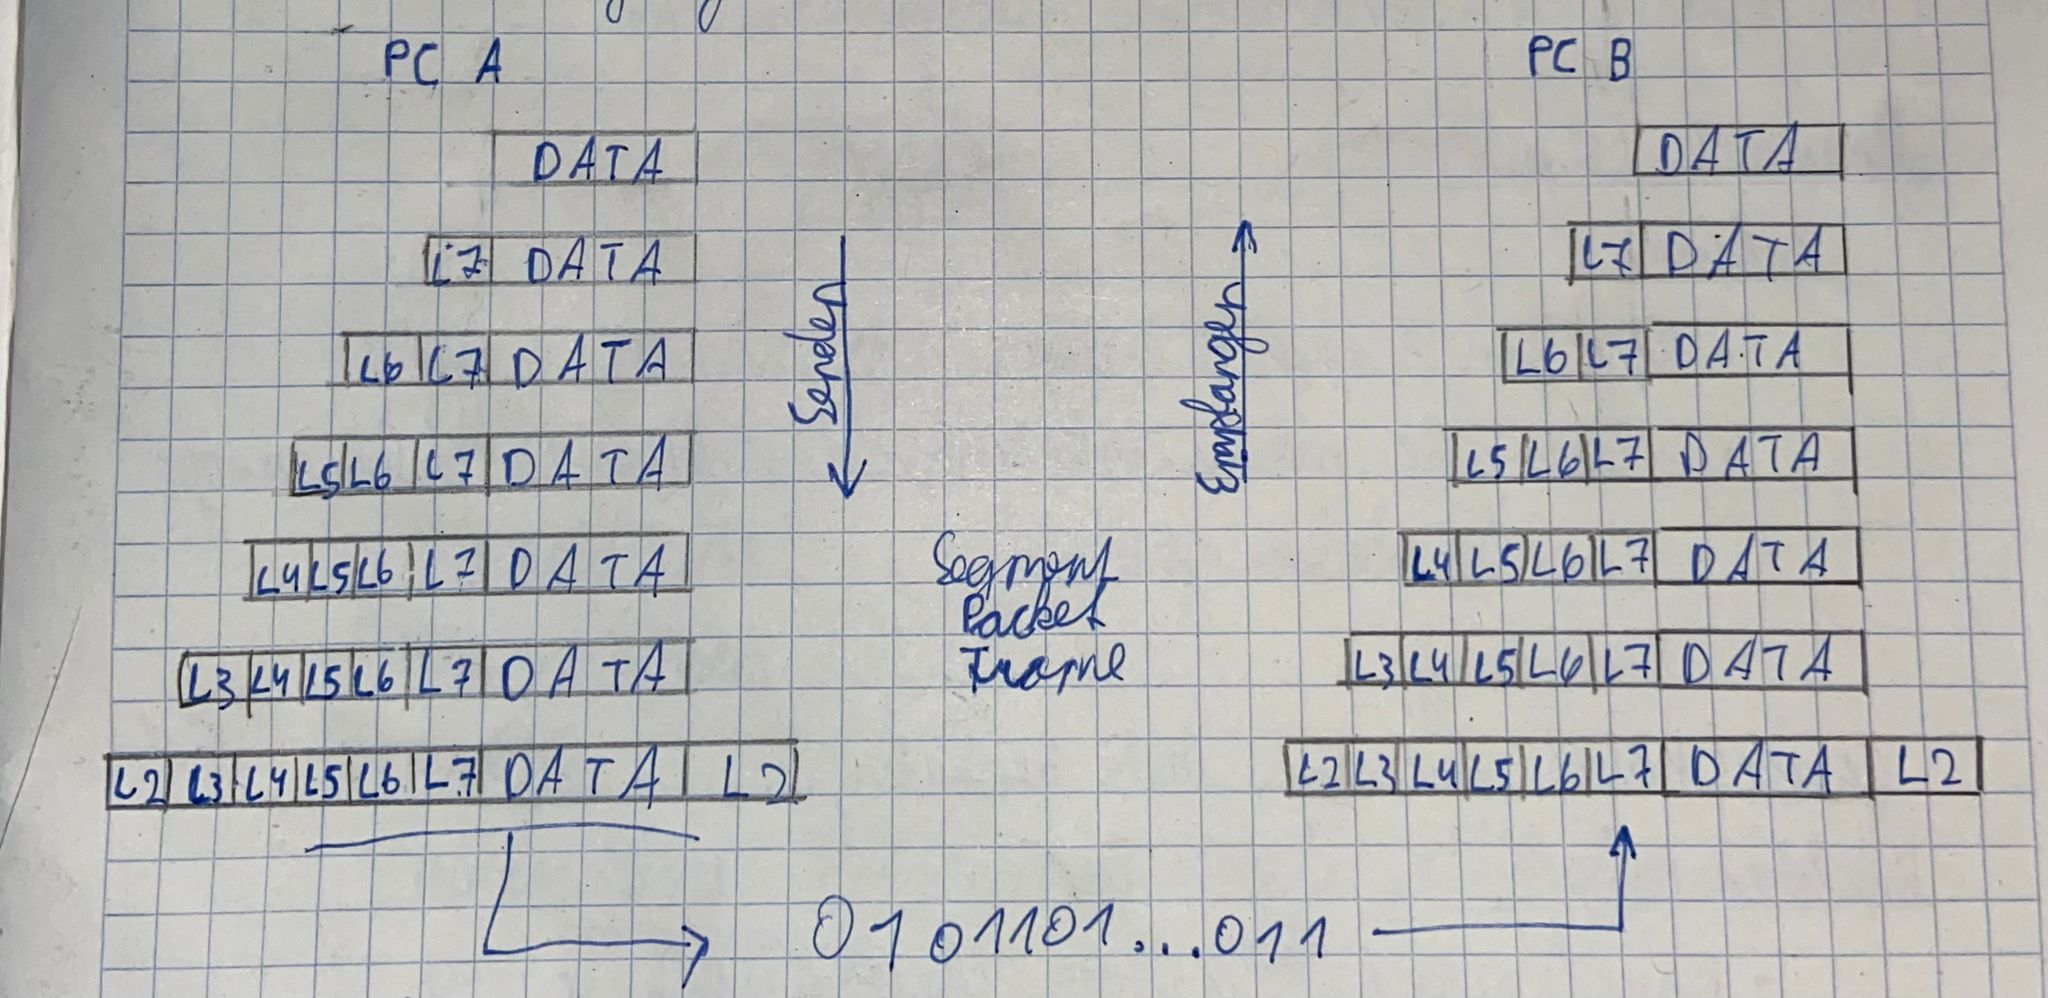
\includegraphics[width=0.9\linewidth]{figures/datenuber.jpeg}
	\caption{OSI-Modell Datenübertragung}
\end{figure}

\textbf{Layer 1 (Physical):} Bits übertragen \\
\textbf{Layer 2 (Data Link):} Lokale Adressierung, Fehlererkennung \\
\textbf{Layer 3 (Network):} Globale Adressierung, Routing \\
\textbf{Layer 4 (Transport):} Datenpaketzuordnung, Segmentierung, Datenfluss steuern \\
\textbf{Layer 5 (Session):} Session Verwalten, Verschlüsselung \\
\textbf{Layer 6 (Presentation):} Darstellung der Daten \\
\textbf{Layer 7 (Application):} Funktionen für die Application \\

%\subsection*{Cisco CLI}
%\begin{figure}[H]
%	\centering
%	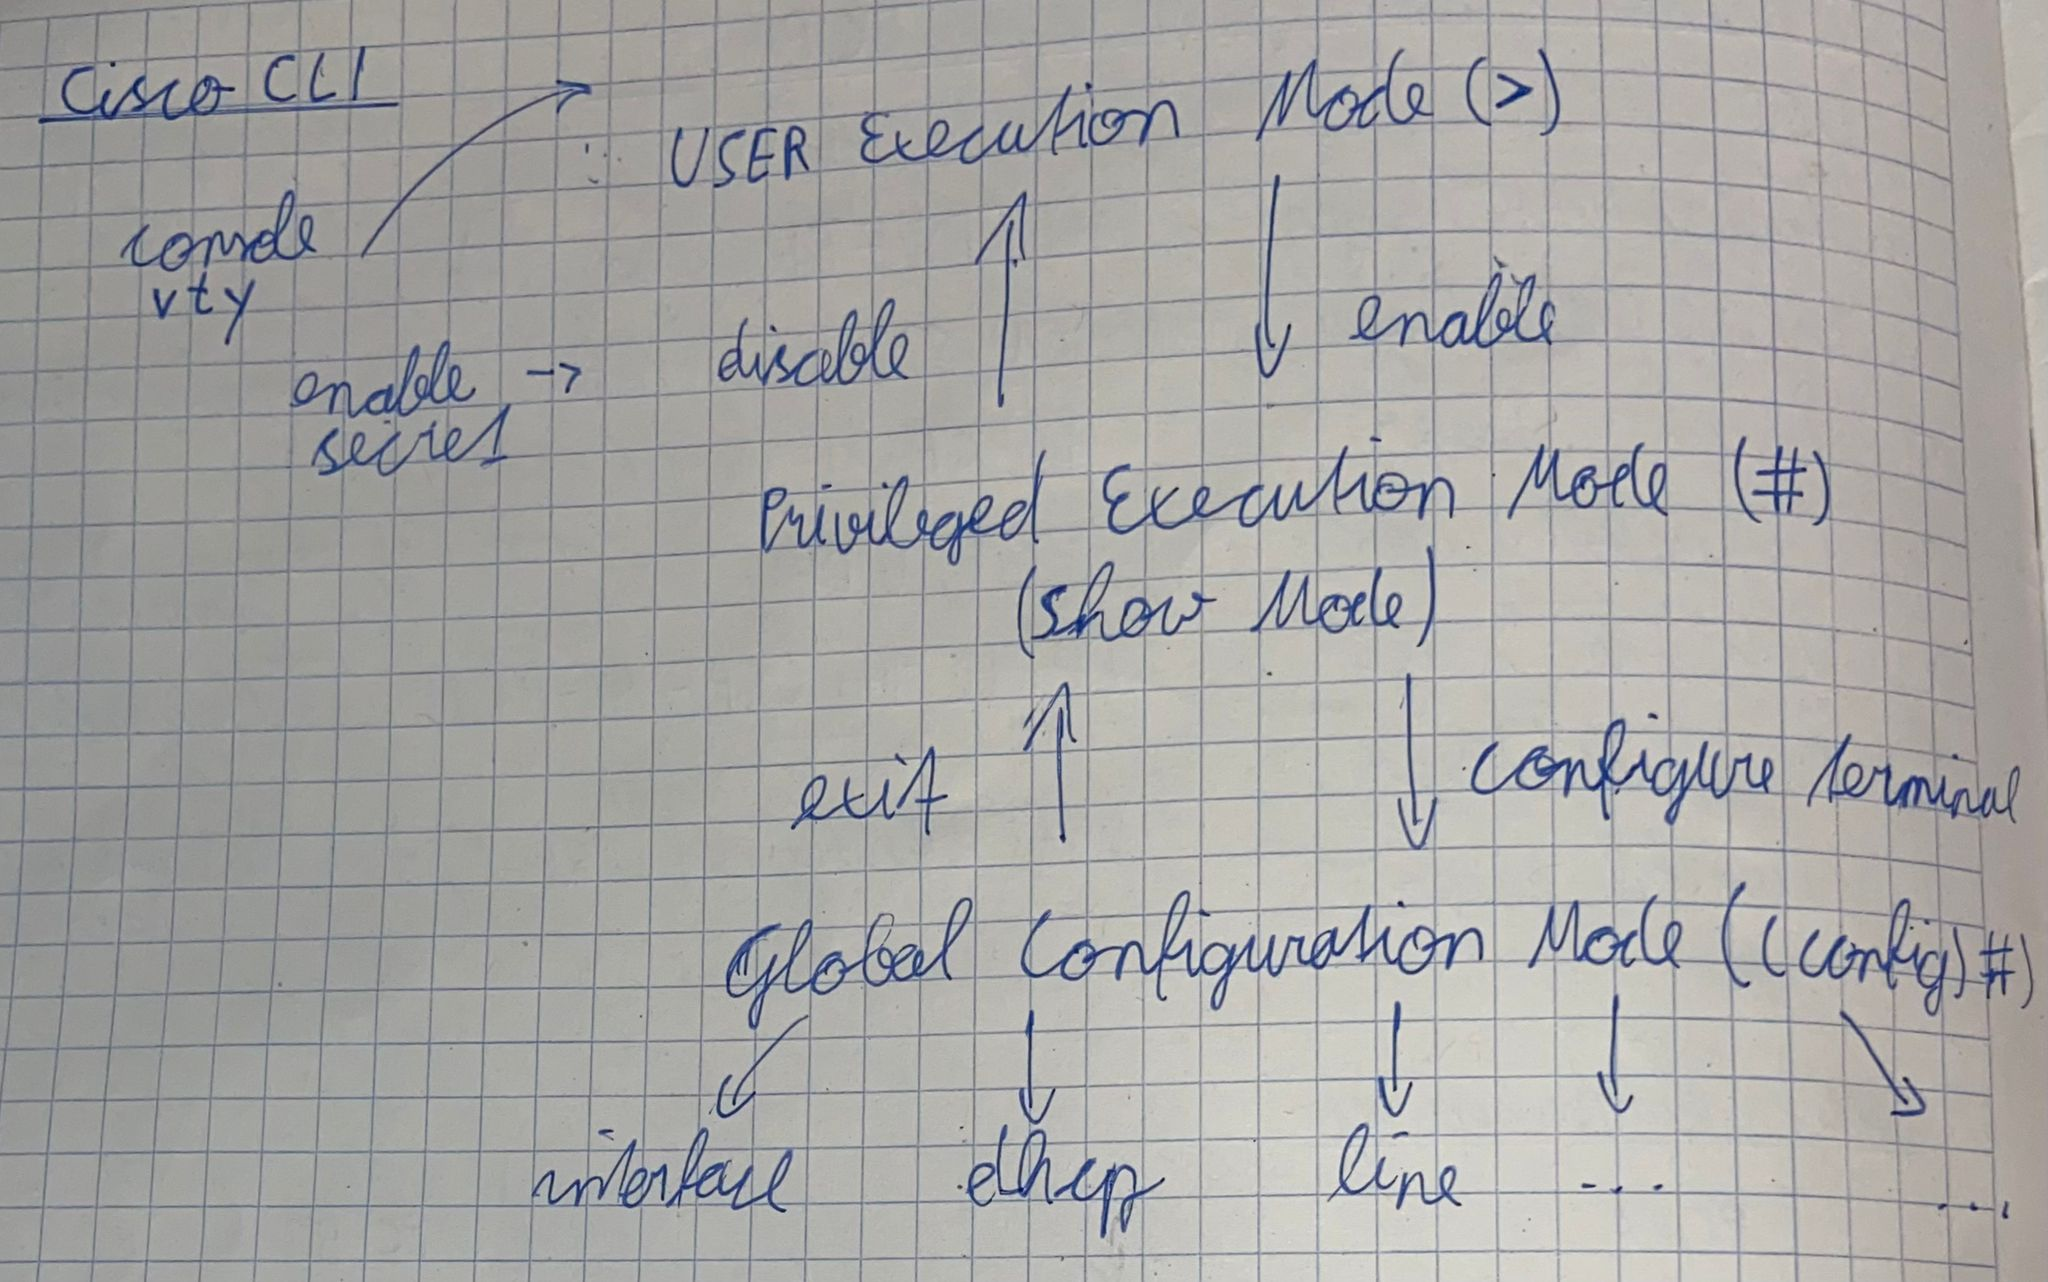
\includegraphics[width=0.9\linewidth]{figures/ciscocli.jpeg}
%	\caption{Cisco CLI}
%\end{figure}
	
	\subsection{Layer 1 (Physical)}
\subsection*{Aufgaben}
\begin{itemize}
	\item Bits von A nach B bringen
	\item elektrische, mechanische oder andere physische Verbindung zwischen zwei Geräten
	\item Kodierung
\end{itemize}
\textbf{Geräte:} Kabel, Antenne, Hub, Repeater,...

\subsection*{Wichtige Begriffe}
\begin{itemize}
	\item Bandbreite (bits/s $\rightarrow$ theoretisch)
	\item Durchsatz (bits/s $\rightarrow$ praktisch)
	\item Latenz (Dauer der Daten von A bis B in ms)
\end{itemize}

\subsection*{Typische Medien}
\begin{itemize}
	\item Kupferkabel (Twisted-Pair-Kabel)
	\item[] \begin{tabbing}
		+ Günstig ~~~~~~~~~~~~~~~~~~~~~ \= $\approx$ Distanz (ca 100m) \\
		+ einfache Handhabung ~~~~ \= $\approx$ Geschwindigkeit \\
		~~~~~~~~~~~~~~~~~~~~~~~~~~~~~~~~~~~~ \= - Interferenzen (Störungen)
	\end{tabbing}
	\begin{itemize}
		\item Straight Through (beide Enden gleich)	
		\item Crossover (verschiedene Enden)
	\end{itemize}
	\item[] (durch Auto MDIX werden Enden automatisch konfiguriert)
	\item Koaxialkabel
	\item Glasfaserkabel
	\begin{tabbing}
		Arten: ~~ \= Single-Mode (Senden Laser, Reichweite 1-10km) \\
		~~~~~~~~~~~ \= Multi-Mode (Senden LED, Reichweite ca 600m)
	\end{tabbing}
	\item[] \begin{figure}[H]
		\centering
		\subfloat[\centering Single-Mode]{{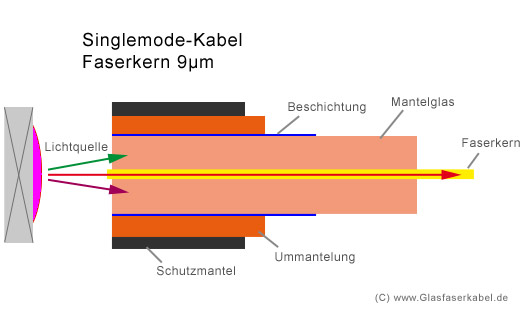
\includegraphics[width=0.46\linewidth]{figures/singlemode.jpg} }}
		\qquad
		\subfloat[\centering Multi-Mode]{{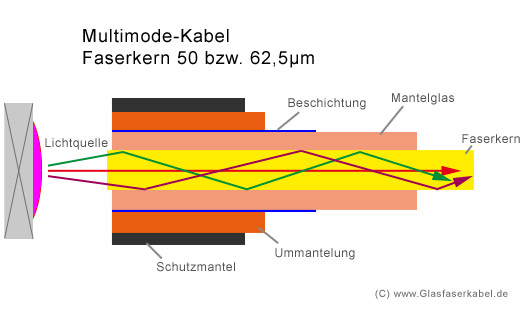
\includegraphics[width=0.46\linewidth]{figures/multimode.jpg} }}
		\caption{Glasfaserkabelarten}
	\end{figure}
	\item[] \begin{tabbing}
		+ Speed ~~~~~~~~~~~~~~~~~ \= - Teuer \\
		+ Reichweite ~~~~~~~~~~~ \= - Handhabung \\
		+ Störungen
	\end{tabbing}
	\item Drahtlos
	\item[] Übertragung: elektromagnetische Wellen über Luft
	\item[] \begin{tabbing}
		+ Flexibel ~~~ \= - Störungen \\
		~~~~~~~~~~~~~~~~~ \= - Shared Medium \\
		~~~~~~~~~~~~~~~~~ \= - Reichweite (ca 100m), Hindernisse \\
		~~~~~~~~~~~~~~~~~ \= - Security \\
	\end{tabbing}
\end{itemize}
	\subsection{Layer 2 (Data Link)}
\subsection*{Aufgaben}
\begin{itemize}
	\item lokale Adressierung
	\item Fehlererkennung
	\item Zugang zum Medium herstellen
	\item Kommunikation mit Layer 3
\end{itemize}

\textbf{Geräte:} Netzwerkkarte, Switch, Bridge,... \\
\textbf{Standards:} Wifi (802.11), Ethernet (802.2, 802.3)
\subsection*{Topologie}
\begin{itemize}
	\item Sterntopologie
	\item Baumtopologie
	\item Punkt-zu-Punkt
\end{itemize}
\begin{figure}[H]
	\centering
	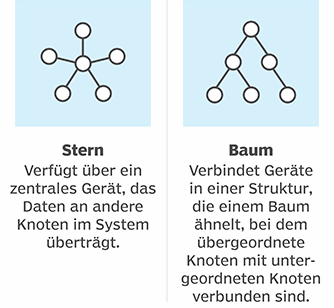
\includegraphics[width=0.6\linewidth]{figures/topologiearten.png}
	\caption{Baum- und Sterntopologie}
\end{figure}

\subsection*{Ethernet}
\begin{figure}[H]
	\centering
	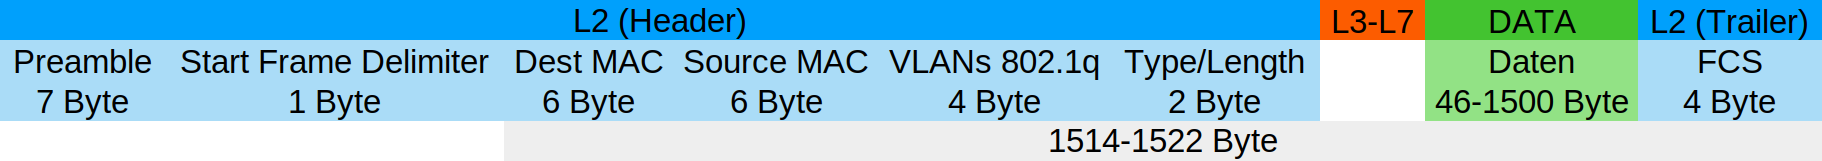
\includegraphics[width=1.0\linewidth]{figures/ethheader.png}
	\caption{Ethernet Frame}
\end{figure}

\subsection*{MAC-Adresse}
Die MAC-Adresse ist eine 48-Bit Zahl und wird in hexadecimal dargestellt.
\begin{tabbing}
	Bsp:\\
	Hersteller ~ \= für den Hersteller einzigartig \\
	DC F5 05 $\vert$\= 17 9A 69 \\
\end{tabbing}

Jede Netzwerkkarte besitzt eine weltweit einzigartige (theoretisch) MAC-Adresse.

\subsection*{Type}
Kodierung für Layer 3 \\
0x800 $\rightarrow$ IP \\
0x806 $\rightarrow$ ARP 

\subsection*{Fehlerkennung}
Frame Checksum (CRC) \\
Polynomdivision mit einem Polynom von Grad 32

\subsection*{Funktion eines Switches}
Der Switch baut mit der Source-MAC seine MAC-Tabelle auf. Dort steht zu jeder MAC-Adresse der passende Port. Falls die MAC-Adresse schon eingetragen ist, wird ein Timer aktualisiert. Sollte es noch keinen Eintrag geben wird er hinzugefügt und bleibt dort eine gewisse Zeit (5 Minuten) bevor er gelöscht wird. Der Switch vergleicht die Destination-MAC mit seiner MAC-Tabelle. Falls der Switch keinen Eintrag findet sendet er an alle Ports (Flooding, Unknown Unicast). Sonst sendet er an den Port, wo er den Frame bekommen hat. \\
Layer 2 Broadcast Adresse: FF:FF:FF:FF:FF:FF

\subsection*{L2, L3 Adressierung}
\begin{figure}[H]
	\centering
	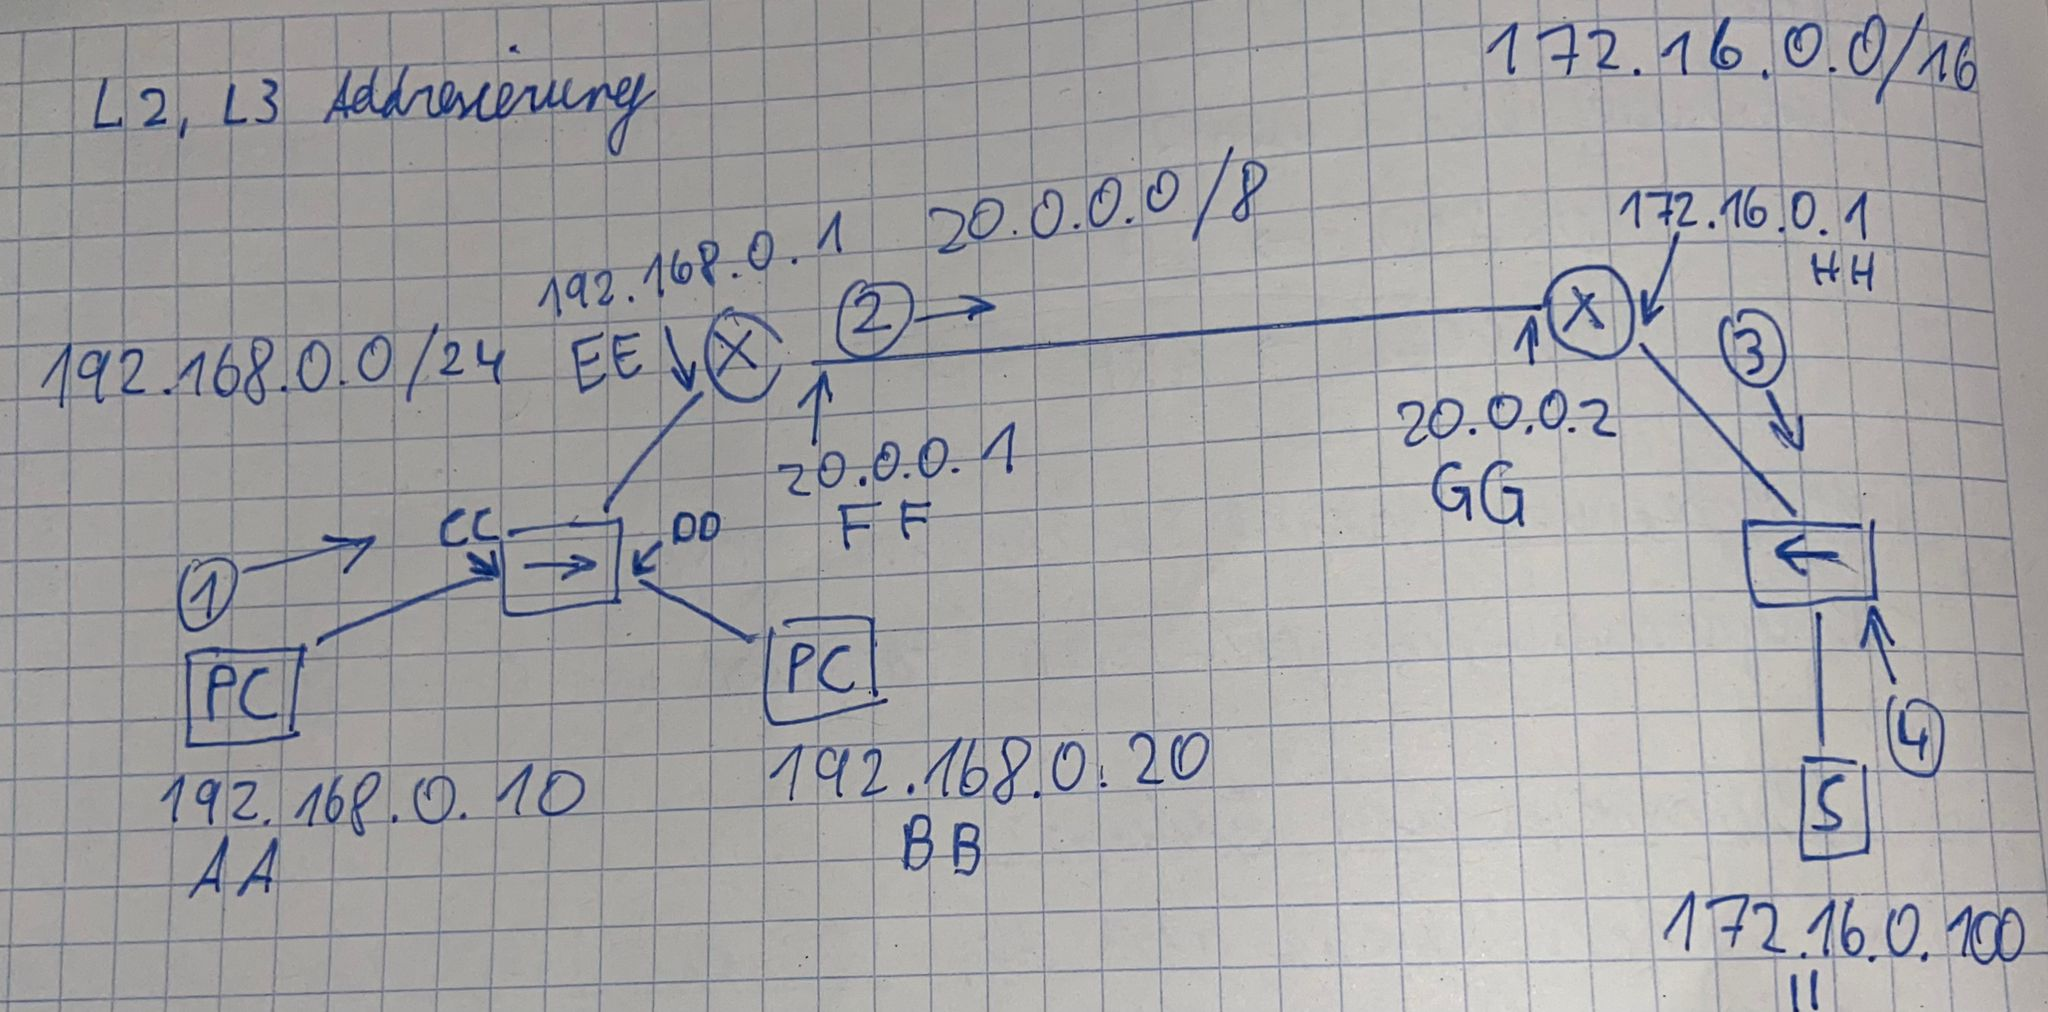
\includegraphics[width=1.0\linewidth]{figures/l2l3add.jpeg}
	\caption{Layer 2 \& 3 Adressierung}
\end{figure}

\begin{table}[H]
	\begin{tabular}{c|cccc}
		& Source MAC & Destination MAC & Source IP & Destination IP \\
		\hline
		1 & AA & EE & 192.168.0.10 & 172.16.0.100 \\
		2 & FF & GG & 192.168.0.10 & 172.16.0.100 \\
		3 & HH & II & 192.168.0.10 & 172.16.0.100 \\
		4 & II & HH & 172.16.0.100 & 192.168.0.10
	\end{tabular}
\end{table}

\subsection*{ARP (Address Resolution Protocol)}
Nutzt ein Host um zu einer gegebenen IP-Adresse die passende MAC-Adresse zu finden

\subsubsection*{ARP-Request (Broadcast)}
Source MAC: eigene MAC-Adresse \\
Destination MAC: FF-FF-FF-FF-FF-FF \\
Type: 0x806
Danach ARP-Header (IP, MAC, Protokoll)

\subsubsection*{ARP-Reply}
Unicast (auch als Broadcast möglich) \\
Source MAC: eigene MAC-Adresse (gesucht) \\
Destination MAC: MAC-Adresse (Anfrage) \\
Type: 0x806 \\
Danach ARP-Header

\subsubsection*{ARP-Cache}
Die Einträge werden im ARP-Cache gespeichert (ca 5 min) \\
IP MAC Time

\subsection*{ARP-Spoofing}
\begin{figure}[H]
	\centering
	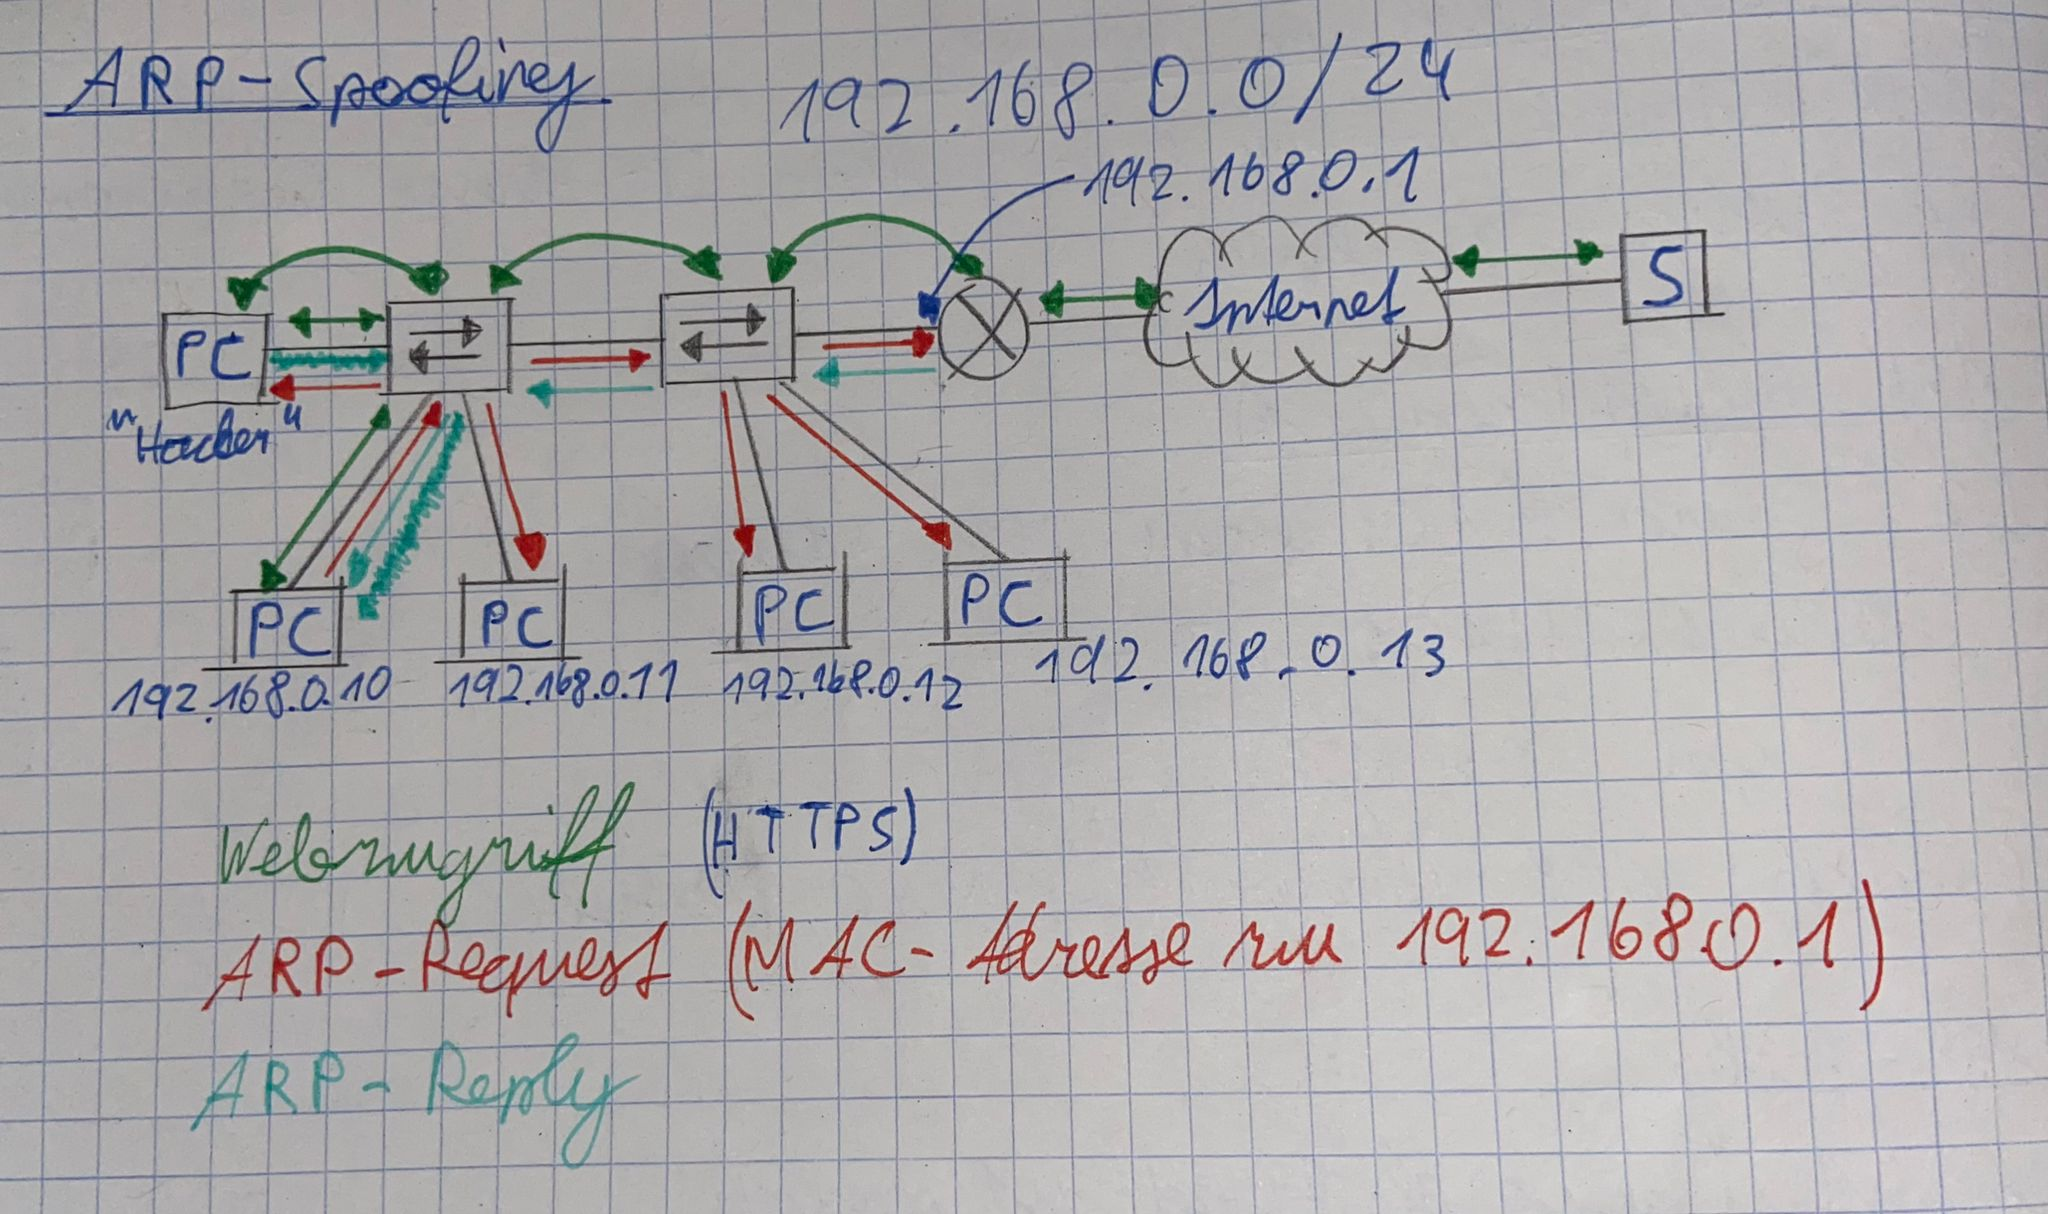
\includegraphics[width=1.0\linewidth]{figures/arpspoofing.jpeg}
	\caption{ARP-Spoofing}
\end{figure}






	\subsection{Layer 3 (Network)}
\subsection*{Aufgaben}
\begin{itemize}
	\item Routing
	\item Globale Adressierung
	\item Kommunikation mit L2 \& L4
\end{itemize}
\textbf{Protkolle:} IPv4, IPv6, ICMP, RIP, OSPF, EIGRP, IS-IS, BGP

\subsection*{IPv4}
Eigenschaften von IP
\begin{itemize}
	\item Verbindungslos
	\item Best Effort
	\item Medium unabhängig
\end{itemize}
\textbf{IP-Header (8.2.2)}
Wichtige Felder: Source \& Destination IP, Time-to-Live

\subsection*{Kommunikationsart}
\begin{itemize}
	\item Unicast (IP des Host)
	\item Multicast (224.0.0.0 - 239.255.255.255)
	\item Broadcast (letzte IP im Netz, 255.255.255.255)
\end{itemize}

\subsection*{Spezielle IP-Adressen}
\begin{itemize}
	\item 127.0.0.0 / 8 ... localhost
	\item 10.0.0.0 / 8
	\item[] 172.16.0.0 / 12
	\item[] 192.168.0.0 / 16 ... private IP-Adressen (NAT)
	\item 169.254.0.0 / 16 ... APIPA
	\item 192.0.2.0 / 24 ... Testnetz
\end{itemize}
\textbf{Fazit:} Zu wenig IPv4-Adressen!

\subsection*{Deshalb}
\begin{itemize}
	\item VLSM (variable length subnet mask)
	\item NAT
	\item IPv6
\end{itemize} 

\subsection*{Classful Addressing (uralt)}
Das erste Oktett bestimmt die Subnetzmaske (/8, /16, /24)
\begin{table}[H]
	\begin{tabular}{ccll}
		Klasse A & 0-127 & (0...) & /8 \\
		Klasse B & 128-191 & (10...) & /16 \\
		Klasse C & 192-223 & (110...) & /24 \\
		Klasse D & 224-239 & (1110...) & Multicast \\
		Klasse E & 240-255 & (11110...) & für spätere Verwendung
	\end{tabular}
\end{table}

\subsection*{Classless Addressing (veraltet!)}
Die Subnetzmasken /8, /16, /24 können beliebig verwendet werden

\subsection*{CIDR (Classless Inter-Domain Routing)}
Es können beliebige Subnetzmasken (z.B. /25, /26, ...) verwendet werden. Alle Subnetze werden gleich groß.

\subsection*{VLSM (variable length subnet mask)}
Alle Subnetzmasken können beliebig verwendet werden. Die Netzte dürfen sich nicht überschneiden.

\subsection*{Subnetzmasken}
\begin{table}[H]
	\begin{tabular}{cccl}
		Präfix Notation & Dotted Decimal Notation & Hosts & Subnetz von /24 \\
		/25 & 255.255.255.128 & $2^{7}$ - 2 = 126 & 2 \\
		/26 & 255.255.255.192 & $2^{6}$ - 2 = 62 & 4 \\
		/27 & 255.255.255.224 & $2^{5}$ - 2 = 30 & 8 \\
		/28 & 255.255.255.240 & $2^{4}$ - 2 = 14 & 16 \\
		/29 & 255.255.255.248 & $2^{3}$ - 2 = 6 & 32 \\
		/30 & 255.255.255.252 & $2^{2}$ - 2 = 2 & 64 \\
		/31 & 255.255.255.254 & $2^{1}$ - 2 = 0 & für spezielle Anwendung \\
		/20 & 255.255.240.0 & $2^{12}$ - 2 = 4.094 & /
	\end{tabular}
\end{table}

\subsection*{Bsp 1 (CIDR):}
\begin{figure}[H]
	\centering
	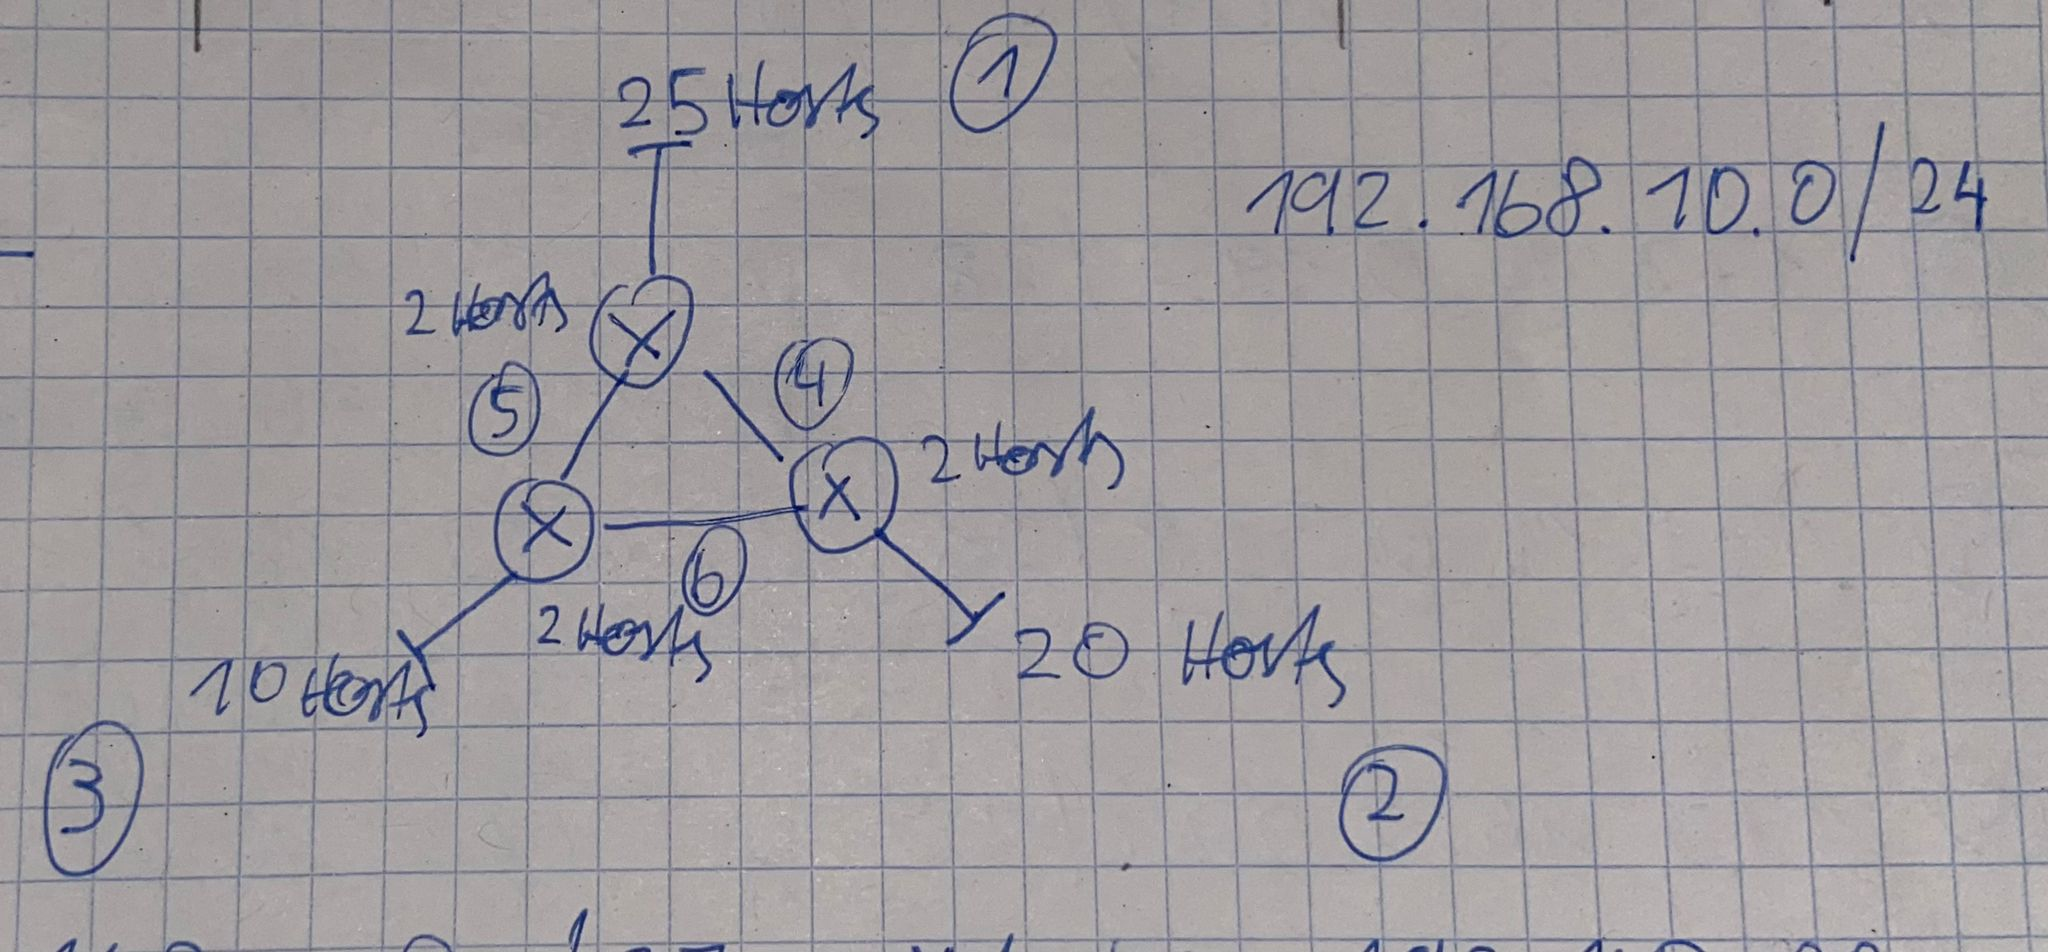
\includegraphics[width=1.0\linewidth]{figures/bsp1_cidr.jpeg}
	\caption{CIDR Beispiel}
\end{figure}
\begin{table}[H]
	\begin{tabular}{llll}
		1 & 192.168.10.0 / 27 & Netzadresse & 192.168.100.0 \\
		&  & Broadcast & 192.168.100.31 \\
		\hline
		2 & 192.168.10.32 / 27 & Netzadresse & 192.168.100.32 \\
		&  & Broadcast & 192.168.100.63 \\
		\hline
		3 & 192.168.10.64 / 27 & Netzadresse & 192.168.100.64 \\
		&  & Broadcast & 192.168.100.95 \\
		\hline
		4 & 192.168.10.96 / 27 & Netzadresse & 192.168.100.96 \\
		&  & Broadcast & 192.168.100.127 \\
		\hline
		5 & 192.168.10.128 / 27 & Netzadresse & 192.168.100.128 \\
		&  & Broadcast & 192.168.100.159 \\
		\hline
		6 & 192.168.10.160 / 27 & Netzadresse & 192.168.100.160 \\
		&  & Broadcast & 192.168.100.191
	\end{tabular}
\end{table}

\subsection*{Bsp 2 (VLSM):}
\begin{figure}[H]
	\centering
	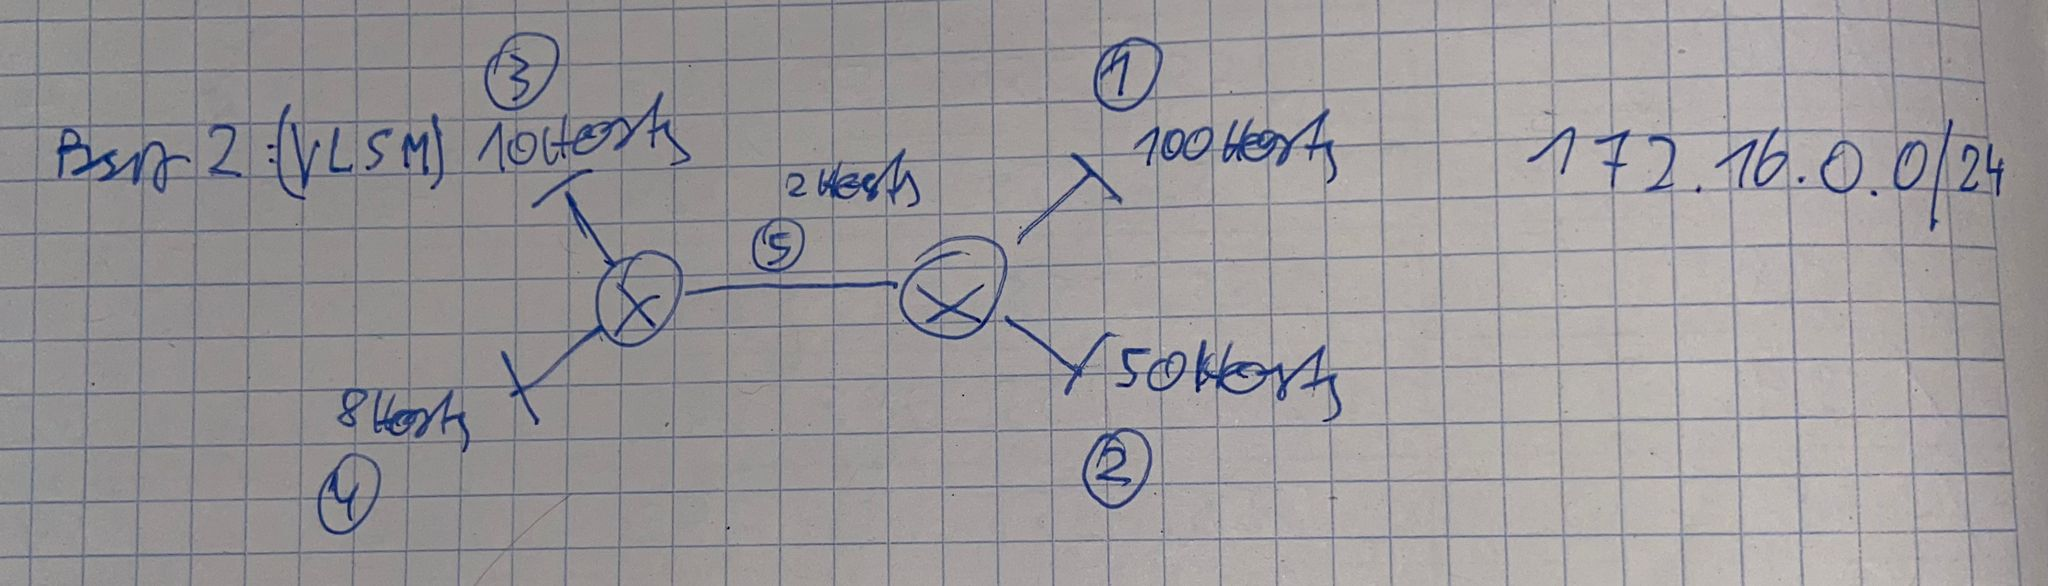
\includegraphics[width=1.0\linewidth]{figures/bsp2_vlsm.jpeg}
	\caption{VLSM Beispiel}
\end{figure}
\begin{table}[H]
	\begin{tabular}{llll}
		1 & 172.16.0.0 / 25 & Netzadresse & 172.16.0.0 \\
		&  & Broadcast & 172.16.0.127 \\
		\hline
		2 & 172.16.0.128 / 26 & Netzadresse & 172.16.0.128 \\
		&  & Broadcast & 172.16.0.191 \\
		\hline
		3 & 172.16.0.192 / 28 & Netzadresse & 172.16.0.192 \\
		&  & Broadcast & 172.16.0.207 \\
		\hline
		4 & 172.16.0.208 / 28 & Netzadresse & 172.16.0.208 \\
		&  & Broadcast & 172.16.0.223 \\
		\hline
		5 & 172.16.0.224 / 30 & Netzadresse & 172.16.0.224 \\
		&  & Broadcast & 172.16.0.227
	\end{tabular}
\end{table}

(PT: 10.4.3, 11.5.5, 11.9.3, 11.10.1)







	\subsection{Layer 4 (Transport)}
\textbf{Aufgaben}
\begin{itemize}
	\item Anwendungen identifizieren
	\item Segmentierung
	\item ev. Flusskontrolle, Verbindungsauf- \& abbau
	\item Kommunikation mit L3 \& L5
\end{itemize}

\textbf{Protkolle:} 
\begin{itemize}
	\item TCP (Transmission Control Protocol)
	\item UDP (User Datagram Protocol)
\end{itemize}

\begin{table}[H]
	\begin{tabular}{l|l}
		\multicolumn{1}{c|}{TCP} & \multicolumn{1}{c}{UDP} \\
		\hline
		Anwendungen identifizieren (Ports) & Anwendungen identifizieren (Ports) \\
		Segmentierung & Segmentierung \\
		Verbindungen auf- bzw abbauen &  \\
		Segmente ordnen &  \\
		wiederholtes Senden &  \\
		Flusskontrolle & 
	\end{tabular}
\end{table}

TCP: HTTP (80)/HTTPS (443), SMTP (25), POP (110), IMAP (143), Telnet (23), SSH (22), FTP (20/21),... \\
UDP: DNS (53), DHCP (67/68), VoIP, Streaming,...

\textbf{Ports} \\
Der Port ist eine 16-Bit Zahl $\rightarrow$ $2^{16} = 65.536$ \\
Der Port identifiziert die Anwendung, sowohl beim Server als auch beim Client.

\textbf{Gruppe von Ports}
\begin{table}[H]
	\begin{tabular}{rc}
		Well-Known-Ports & 0 - 1.023 \\
		Registered-Ports & 1.024 - 49.151 \\
		Private Ports & 49.152 - 65.535
	\end{tabular}
\end{table}

\textbf{L4-Adressierung}
\begin{figure}[H]
	\centering
	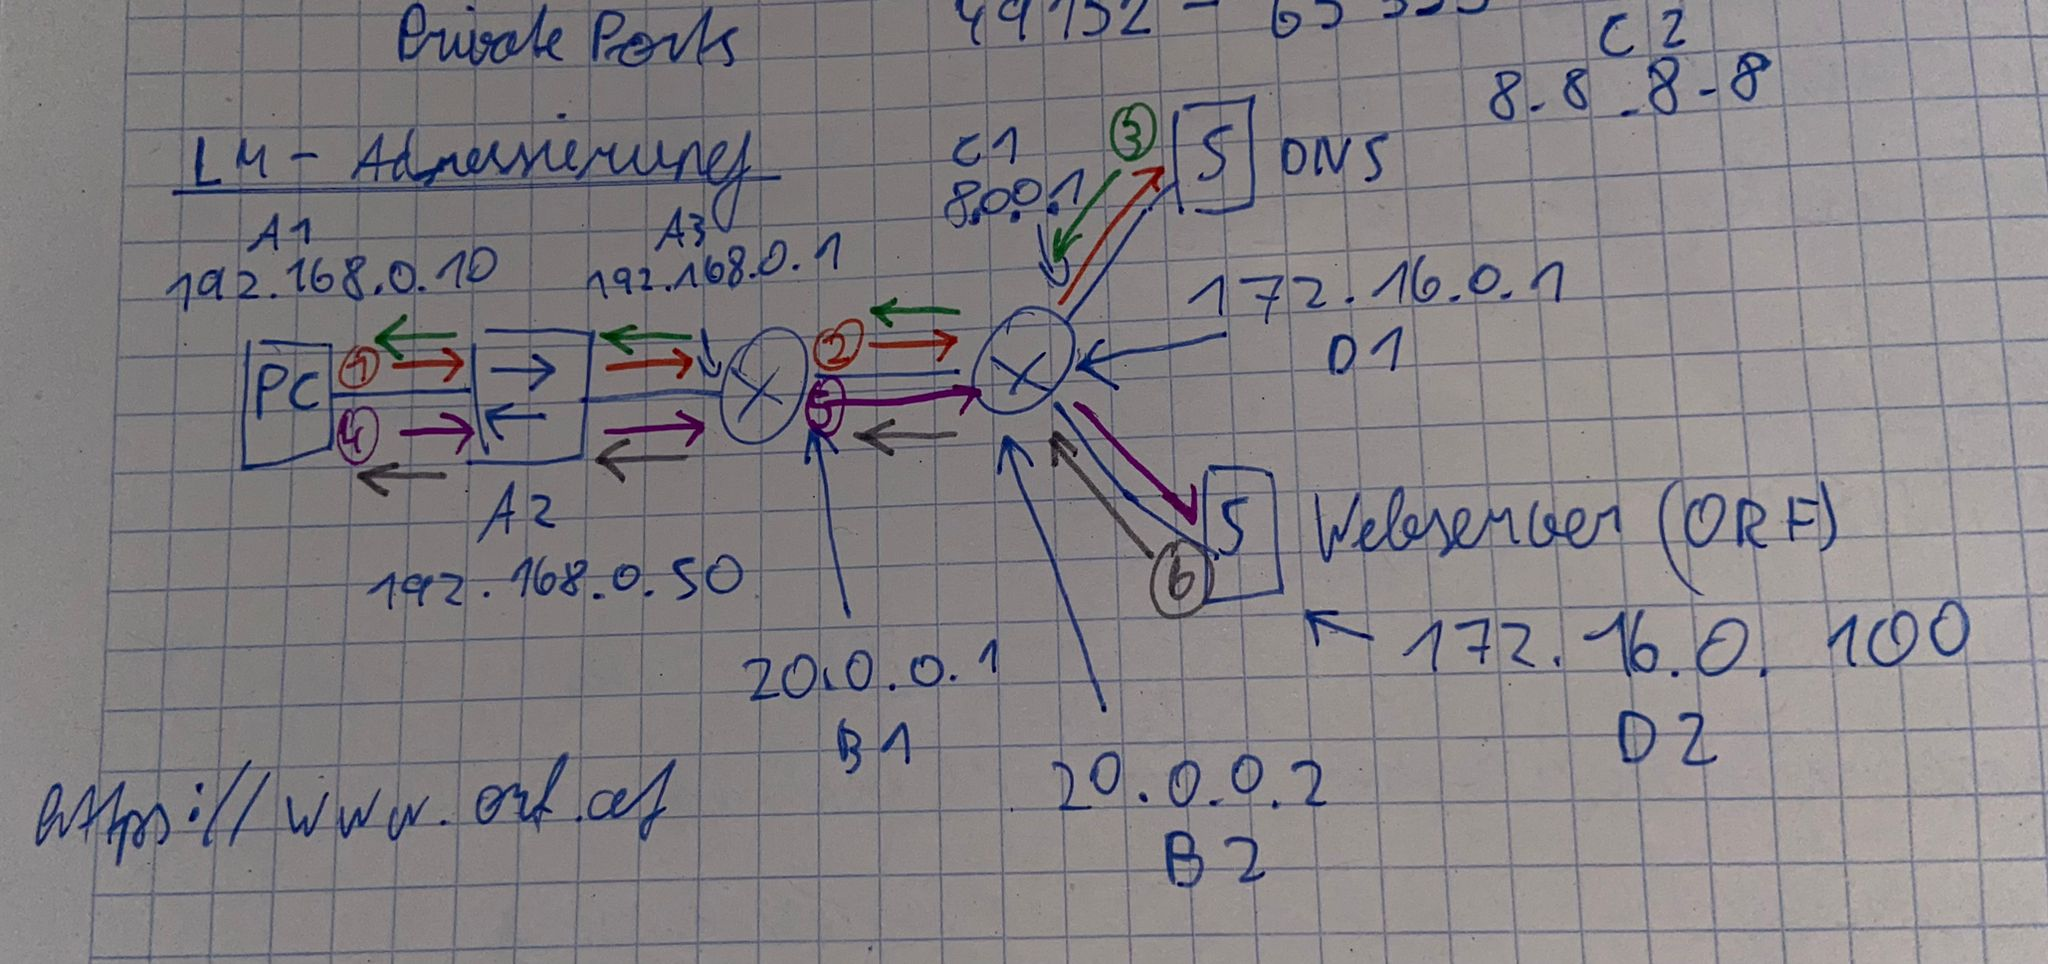
\includegraphics[width=1.0\linewidth]{figures/l4_addr.jpeg}
	\caption{L4-Adressierung}
	\label{fig:l4_addr}
\end{figure}

\begin{table}[H]
	\begin{tabular}{c|ccllll}
		& \multicolumn{2}{c}{L2 (MAC)} & \multicolumn{2}{c}{L3 (IP)} & \multicolumn{2}{c}{L4 (Ports)} \\
		& \multicolumn{1}{c}{Source} & \multicolumn{1}{c}{Destination} & \multicolumn{1}{c}{Source} & \multicolumn{1}{c}{Destination} & \multicolumn{1}{c}{Source} & \multicolumn{1}{c}{Destination} \\
		\hline
		1 & A1 & A3 & 192.168.0.10 & 8.8.8.8 & 53.722 & 53 \\
		2 & B1 & B2 & 192.168.0.10 & 8.8.8.8 & 53.722 & 53 \\
		3 & C2 & C1 & 8.8.8.8 & 192.168.0.10 & 53 & 53.722 \\
		4 & A1 & A3 & 192.168.0.10 & 172.16.0.100 & 60.112 & 443 \\
		5 & B1 & B2 & 192.168.0.10 & 172.16.0.100 & 60.112 & 443 \\
		6 & D2 & D1 & 172.16.0.100 & 192.168.0.10 & 443 & 60.112
	\end{tabular}
\end{table}

\textbf{TCP} \\
Verbindungsaufbau: Drei-Wege-Handshake
\begin{figure}[H]
	\centering
	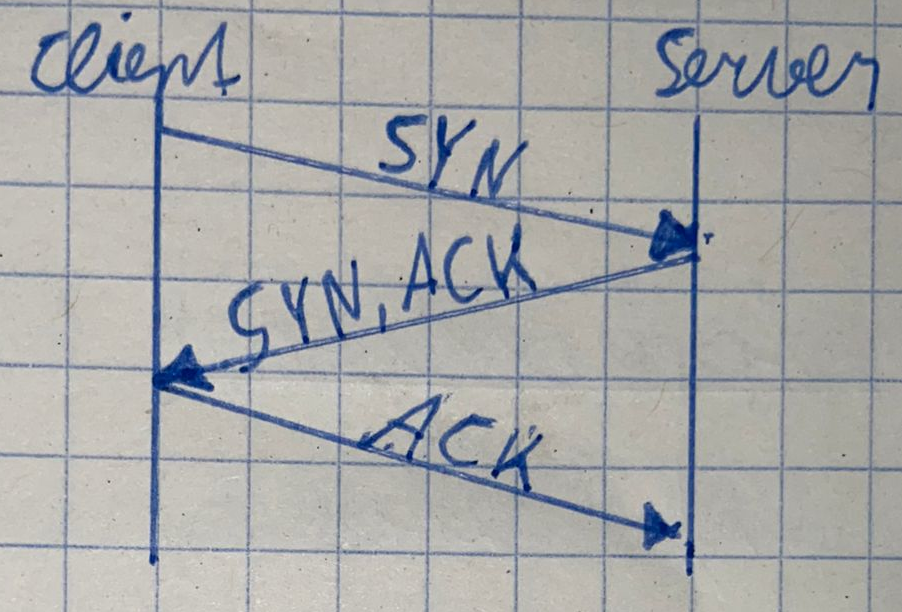
\includegraphics[width=0.8\linewidth]{figures/tcp_3wh.png}
	\caption{TCP 3-Way-Handshake}
\end{figure}

Verbindungsabbau: Zwei-Wege-Handshake
\begin{figure}[H]
	\centering
	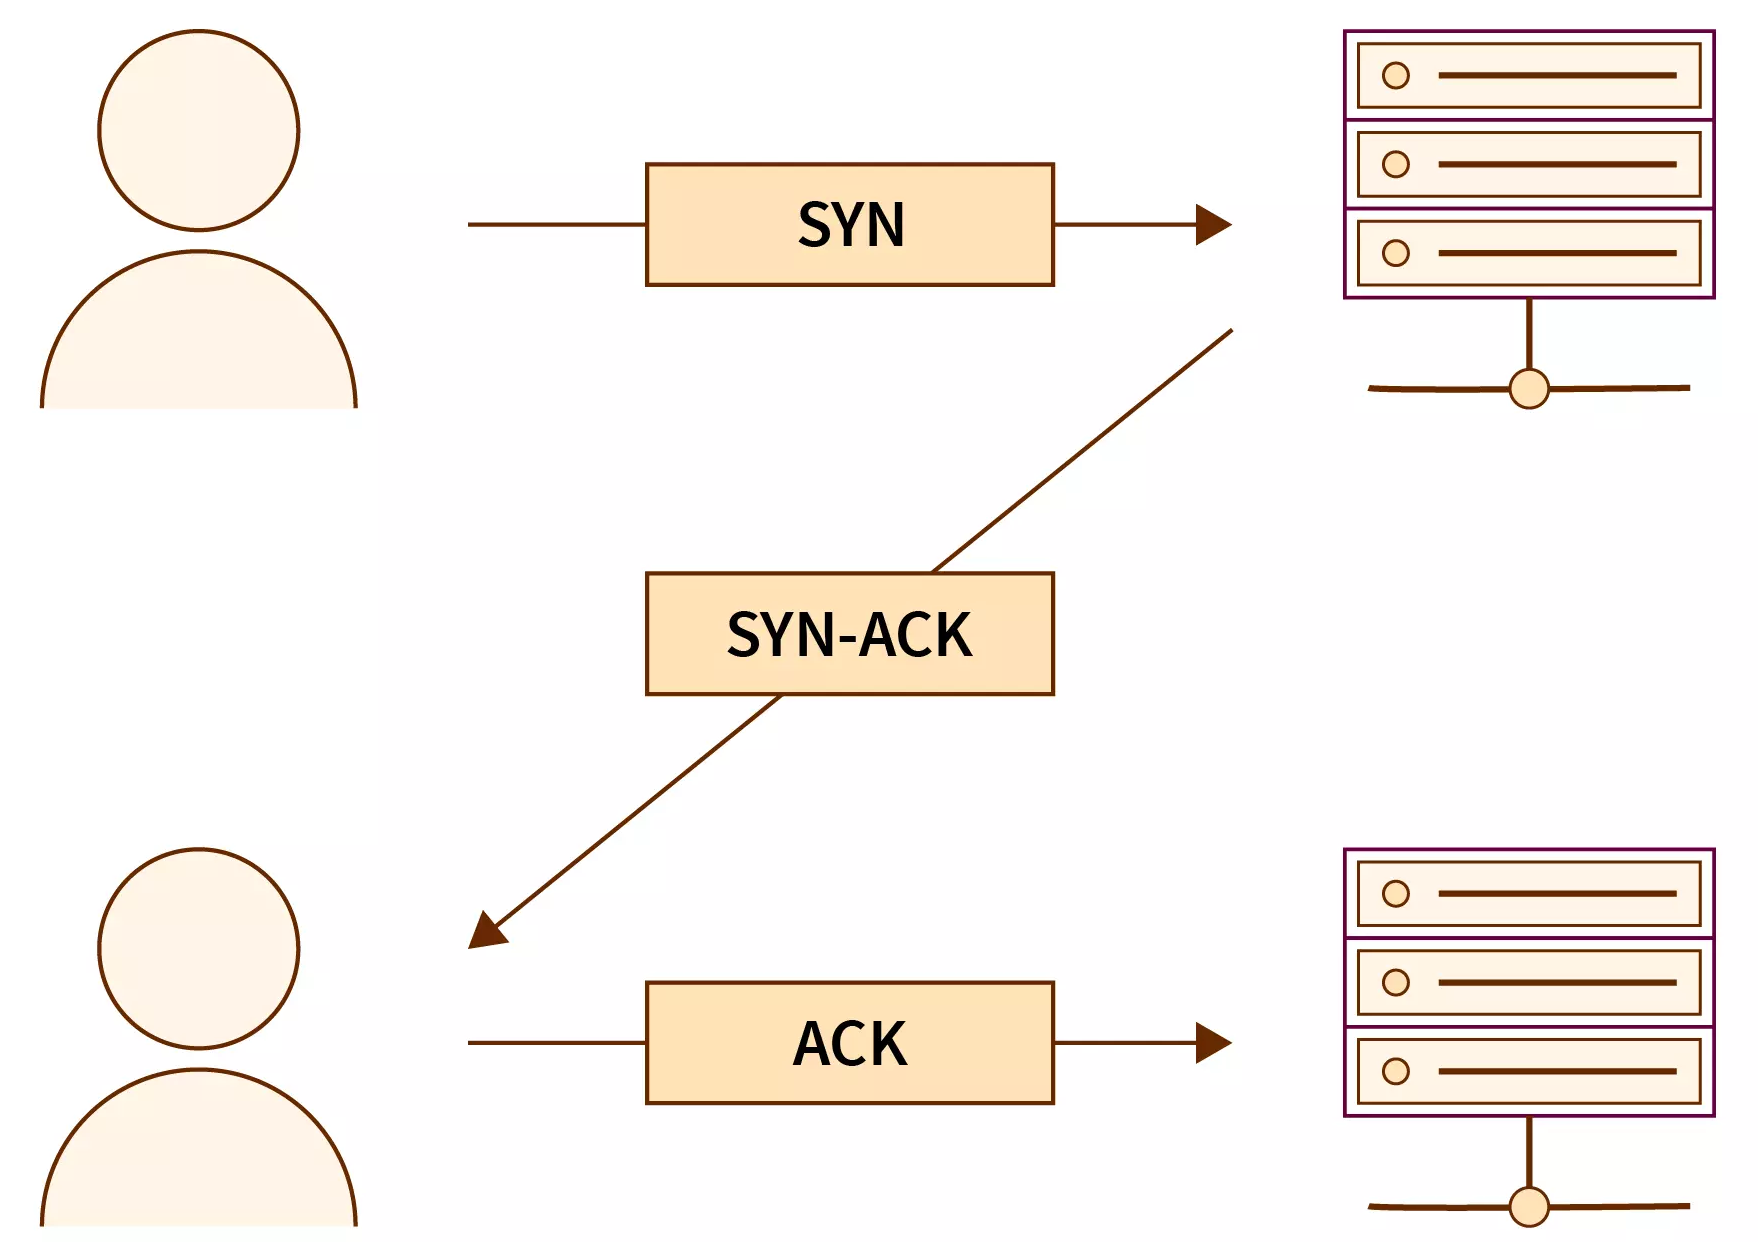
\includegraphics[width=0.8\linewidth]{figures/tcp_2wh.png}
	\caption{TCP 2-Way-Handshake}
\end{figure}

\textbf{Segmentierung} \\
Es wird eine SEQUENCENUMBER mitgeschickt. Diese gibt die Reihenfolge an. Der Client bestätigt die Segmente mit ACK-Segmente. Die ACK-NUMBER gibt an, welches Segment als nächstes kommen soll.
\begin{figure}[H]
	\centering
	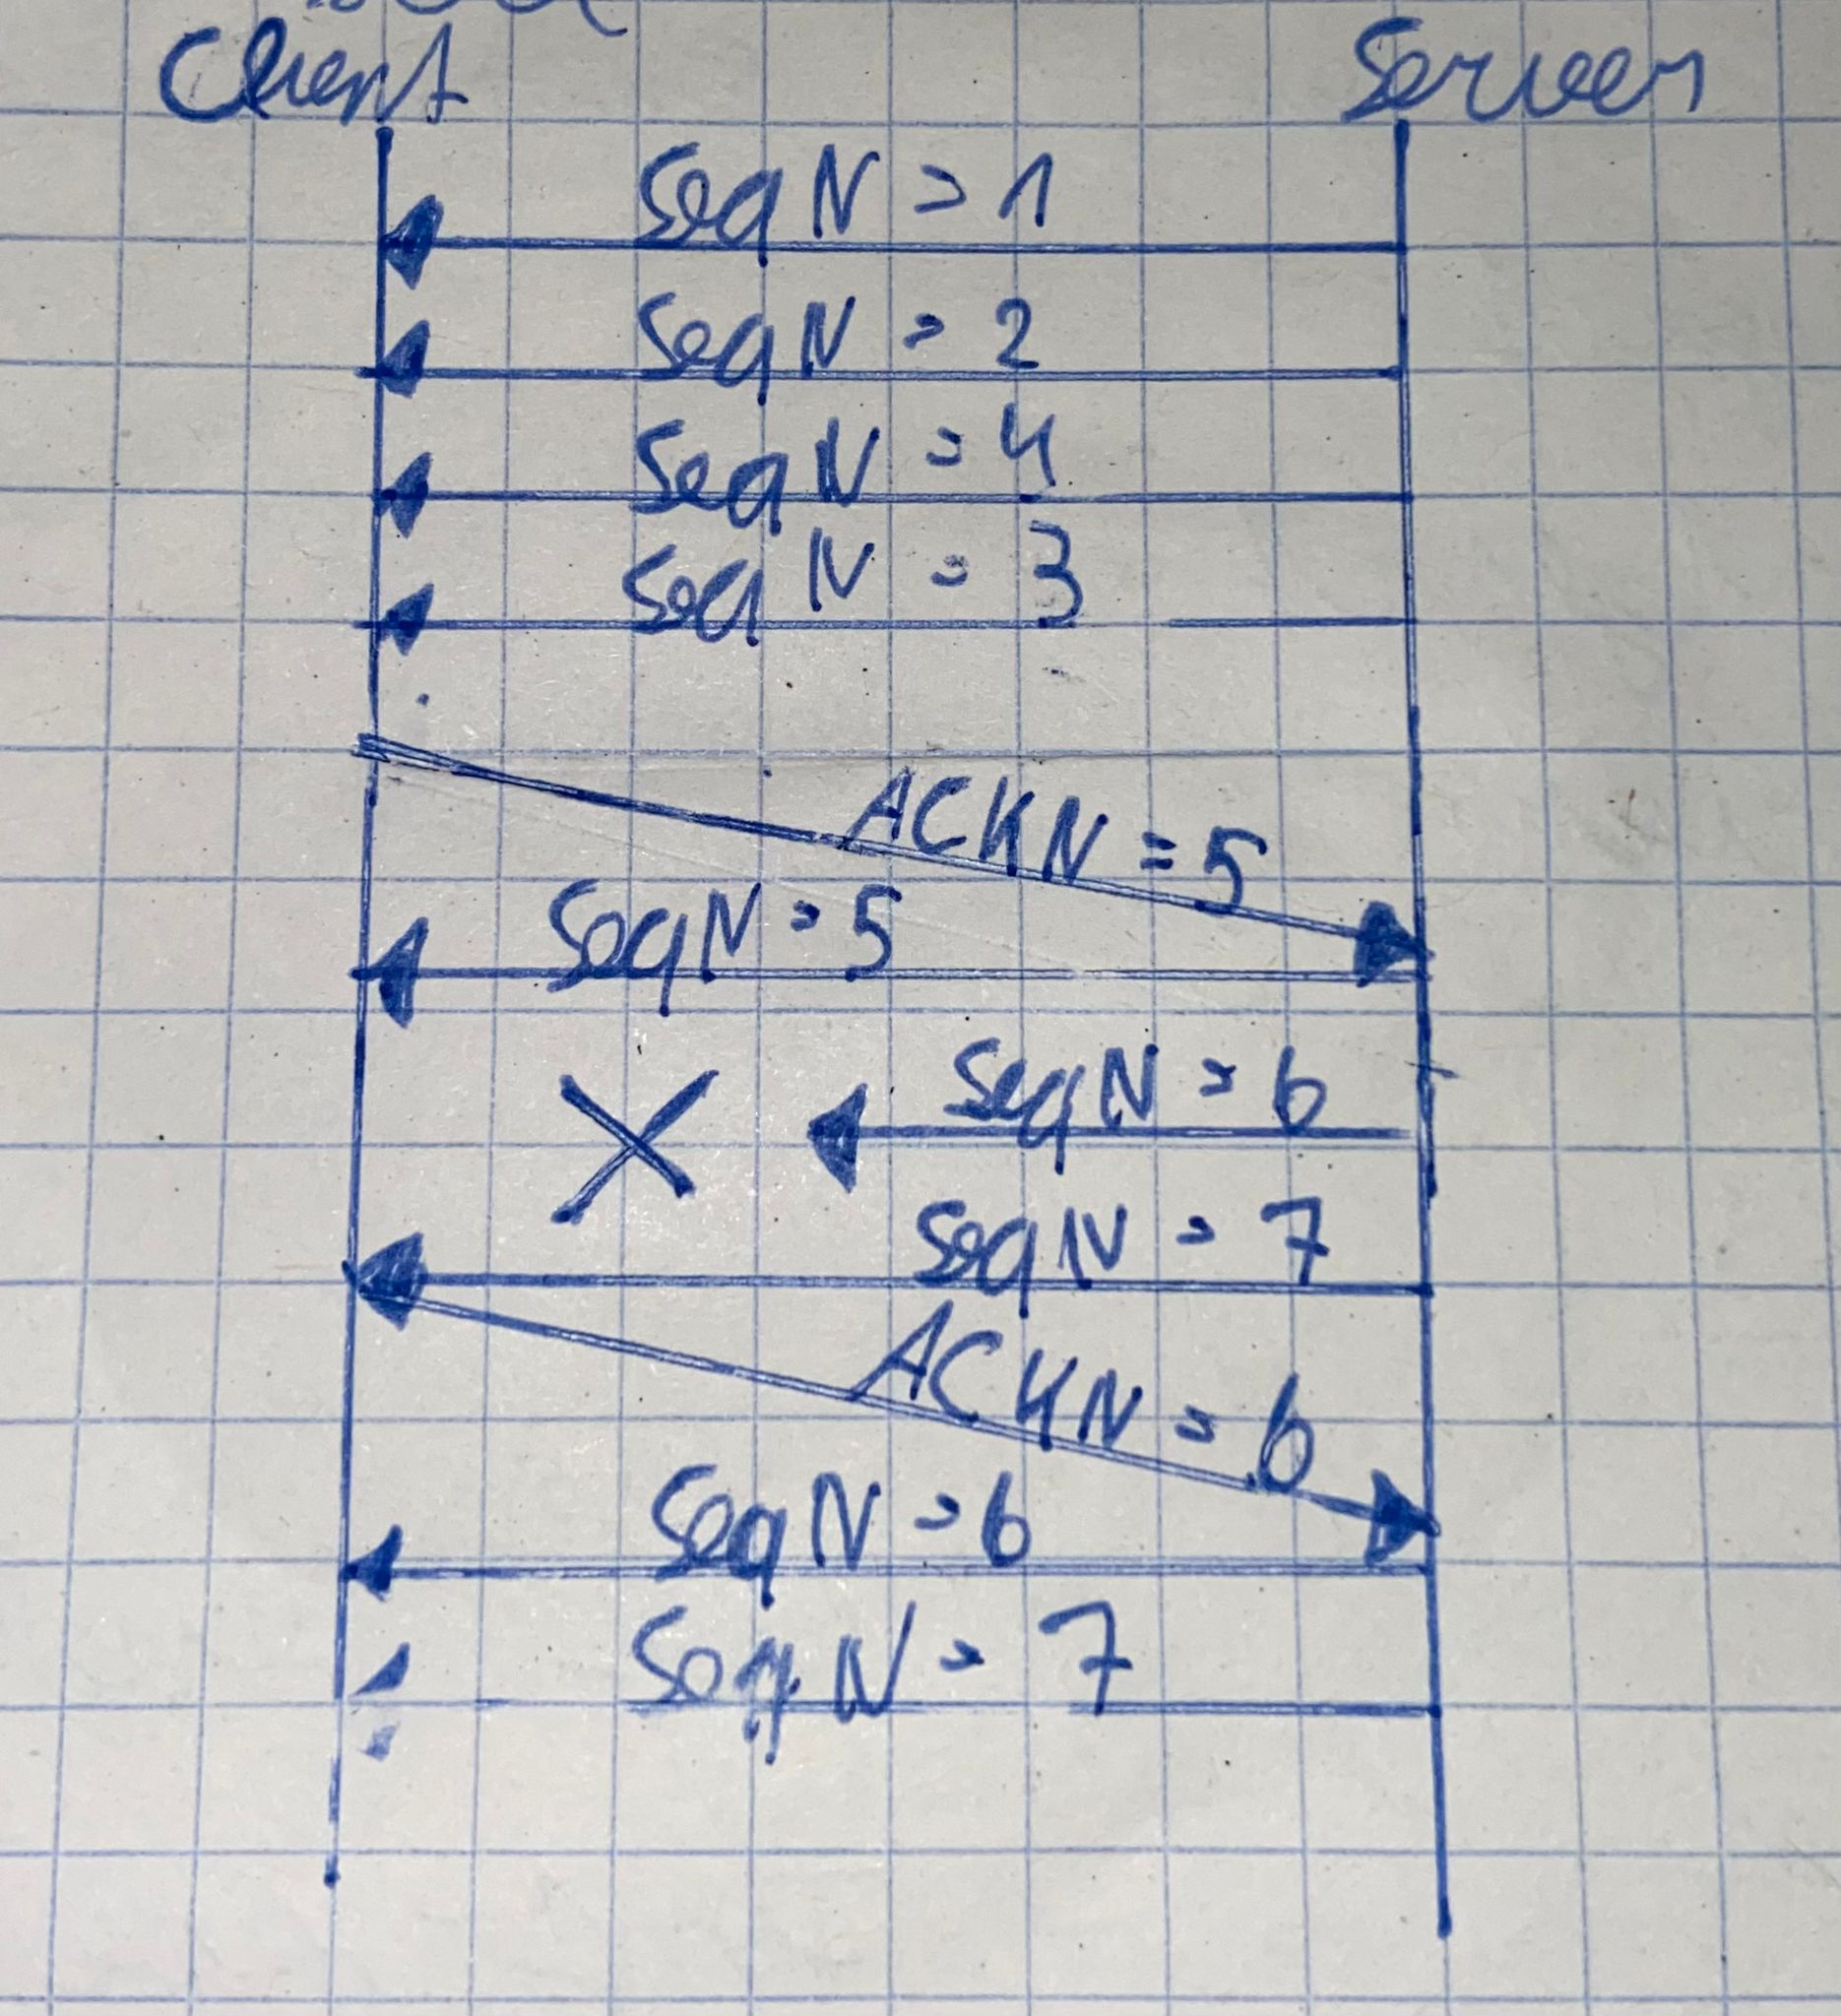
\includegraphics[width=0.8\linewidth]{figures/l4_segment.jpeg}
	\caption{Layer 4 Segmentierung}
\end{figure}

\textbf{Flow-Control} \\
Die Window Size gibt an wann das nächste ACK-Segment erwartet wird.

	\subsection{Layer 5, 6, 7 (Session, Presentation, Application)}
\subsection*{Aufgaben}
\begin{itemize}
	\item Session erstellen und halten
	\item Regelung der Session, Restart, Exchange, Idle
	\item Format und Präsentation der Daten
	\item Verschlüsselung und Komprimierung der Daten
	\item Anwendungsspezifische Informationen
\end{itemize}
\textbf{Protokolle:} HTTP/HTTPS, FTP, Telnet/SSH, DHCP, DNS, SMTP, POP, IMAP

\subsection*{DNS (Port 53, UDP)}
Um zu einer Domain die passende IP-Adresse zu finden.
Typische DNS-Server: 8.8.8.8

\begin{figure}[H]
	\centering
	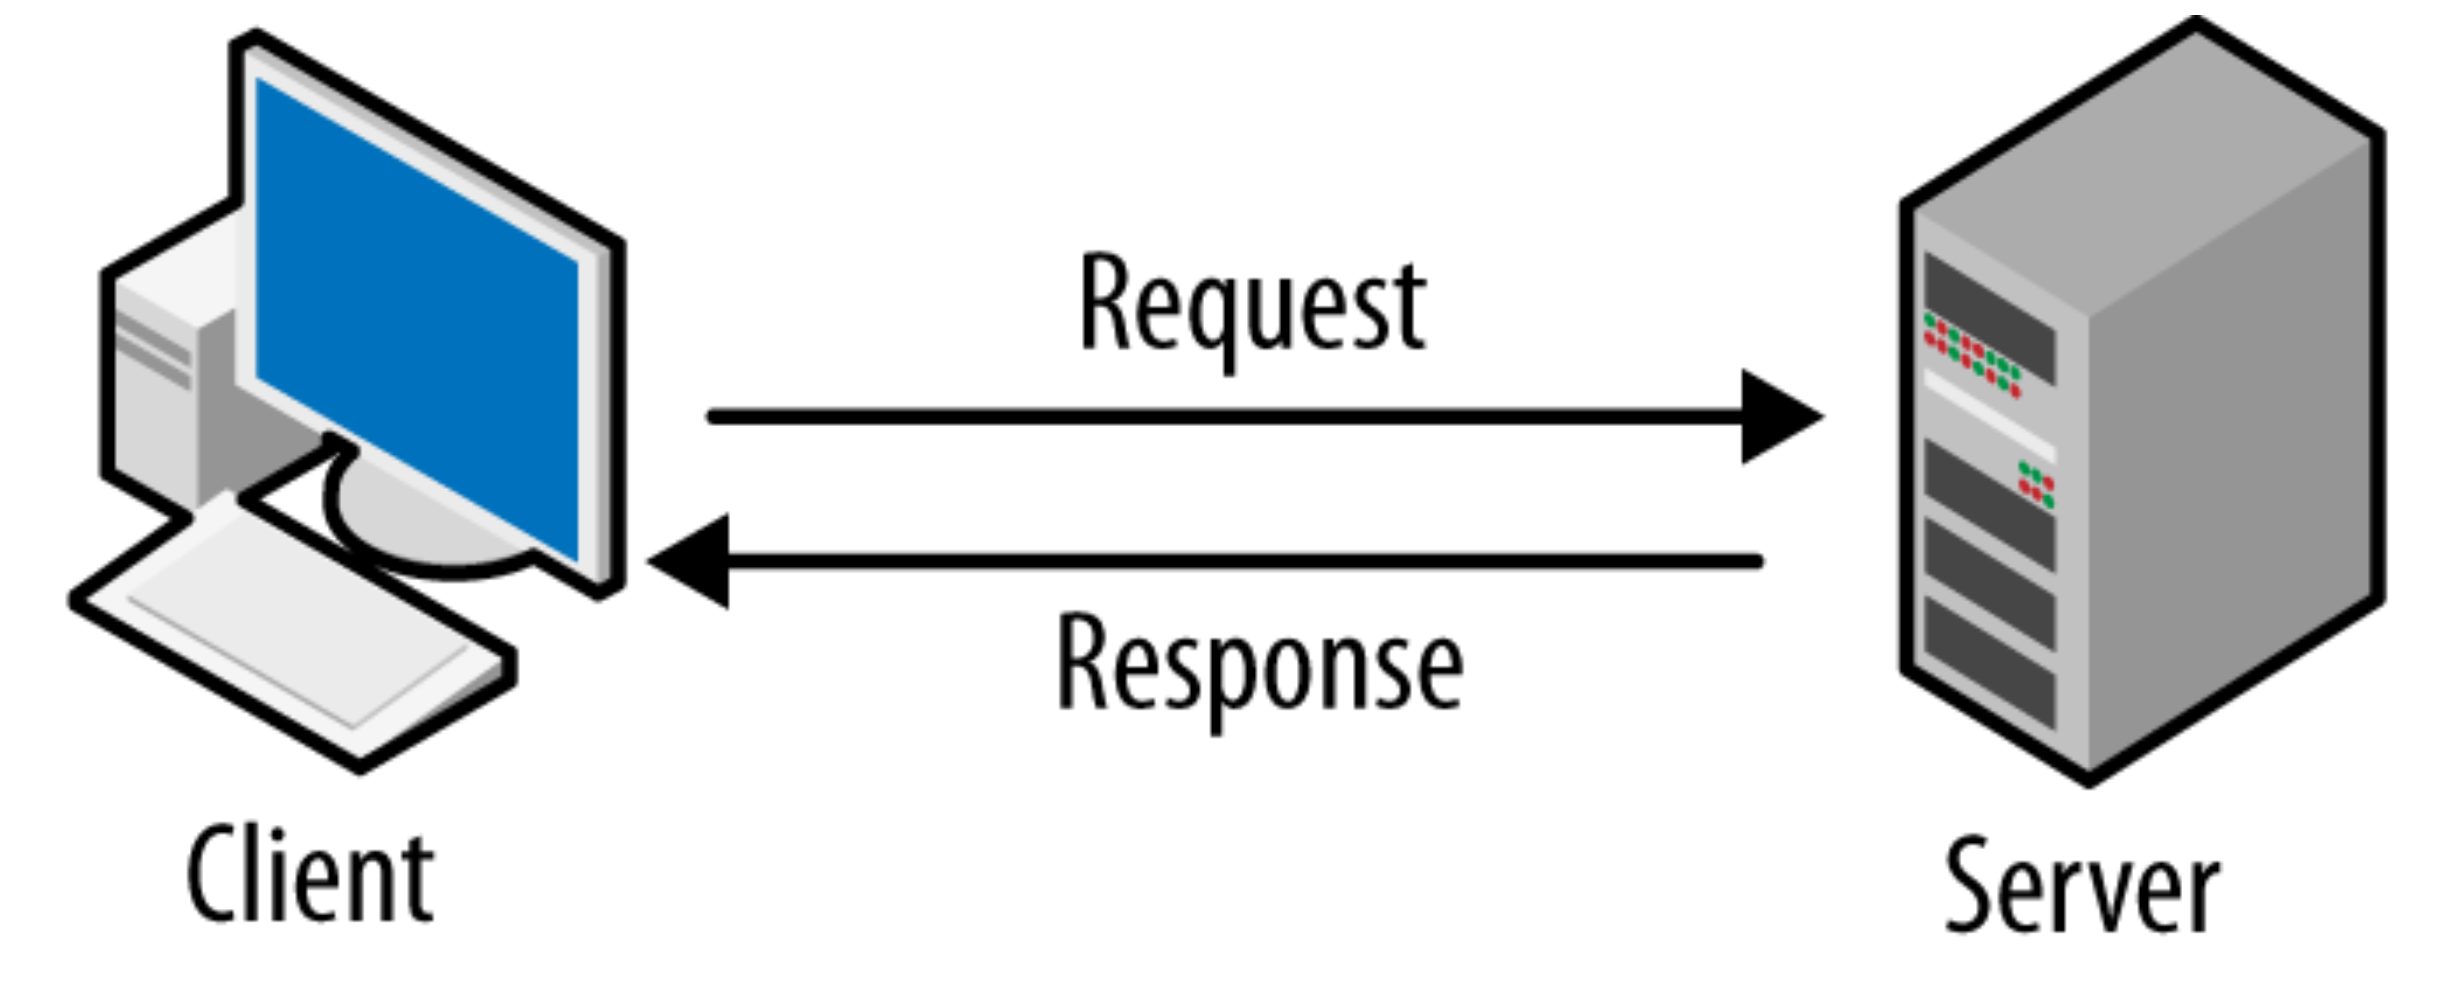
\includegraphics[width=0.8\linewidth]{figures/request_response.png}
	\caption{Request/Response Modell}
\end{figure}

\subsection*{Einträge}
A ... IPv4-Endgerät \\
AAAA ... IPv6-Endgerät \\
MX ... Mail-Server

\subsection*{Hierarchisches DNS-Modell}
\begin{figure}[H]
	\centering
	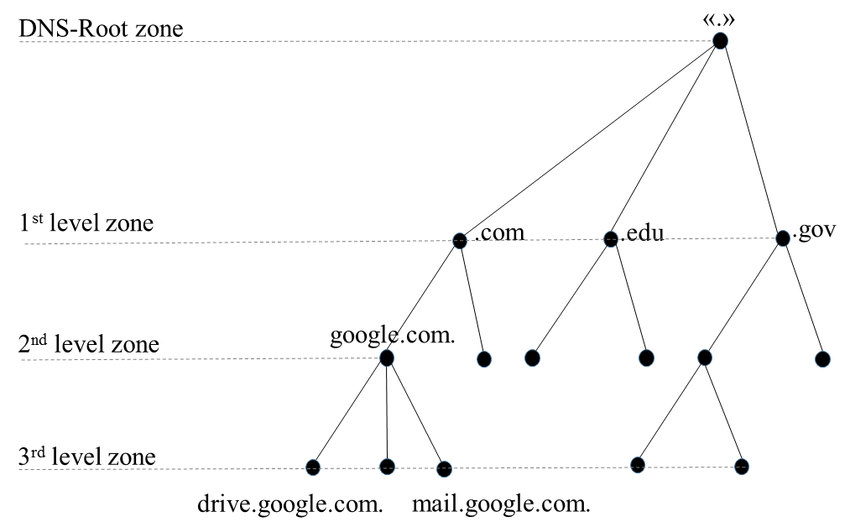
\includegraphics[width=0.8\linewidth]{figures/dns_hierarchy.png}
	\caption{DNS-Hierarchie}
\end{figure}
Falls der DNS-Server keinen Eintrag findet, wird das Paket weitergeleitet. Der Client speichert die erhaltenen DNS-Einträge.

\subsection*{DHCP (Port 67/68, UDP)}
Die Hosts erhalten dynamisch eine IP-Konfiguration (IP-Adresse, Subnetzmaske, Default Gateway, DNS-Server, Lease Time,...).

\begin{figure}[H]
	\centering
	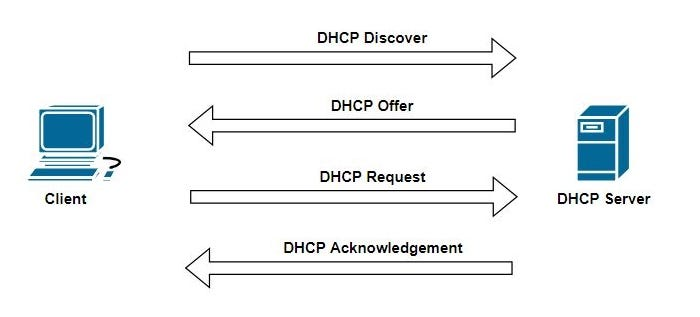
\includegraphics[width=0.8\linewidth]{figures/dhcp_handshake.jpg}
	\caption{DHCP-Handshake}
\end{figure}
DHCP-Discover ... Broadcast \\
DHCP-Offer ... Unicast \\
DHCP-Request ... Broadcast \\
DHCP-ACK ... Unicast \\ 
\textbf{Achtung:} DHCP-Spoofing

\subsection*{HTTP/HTTPS (Port 80/443, TCP)}
\begin{figure}[H]
	\centering
	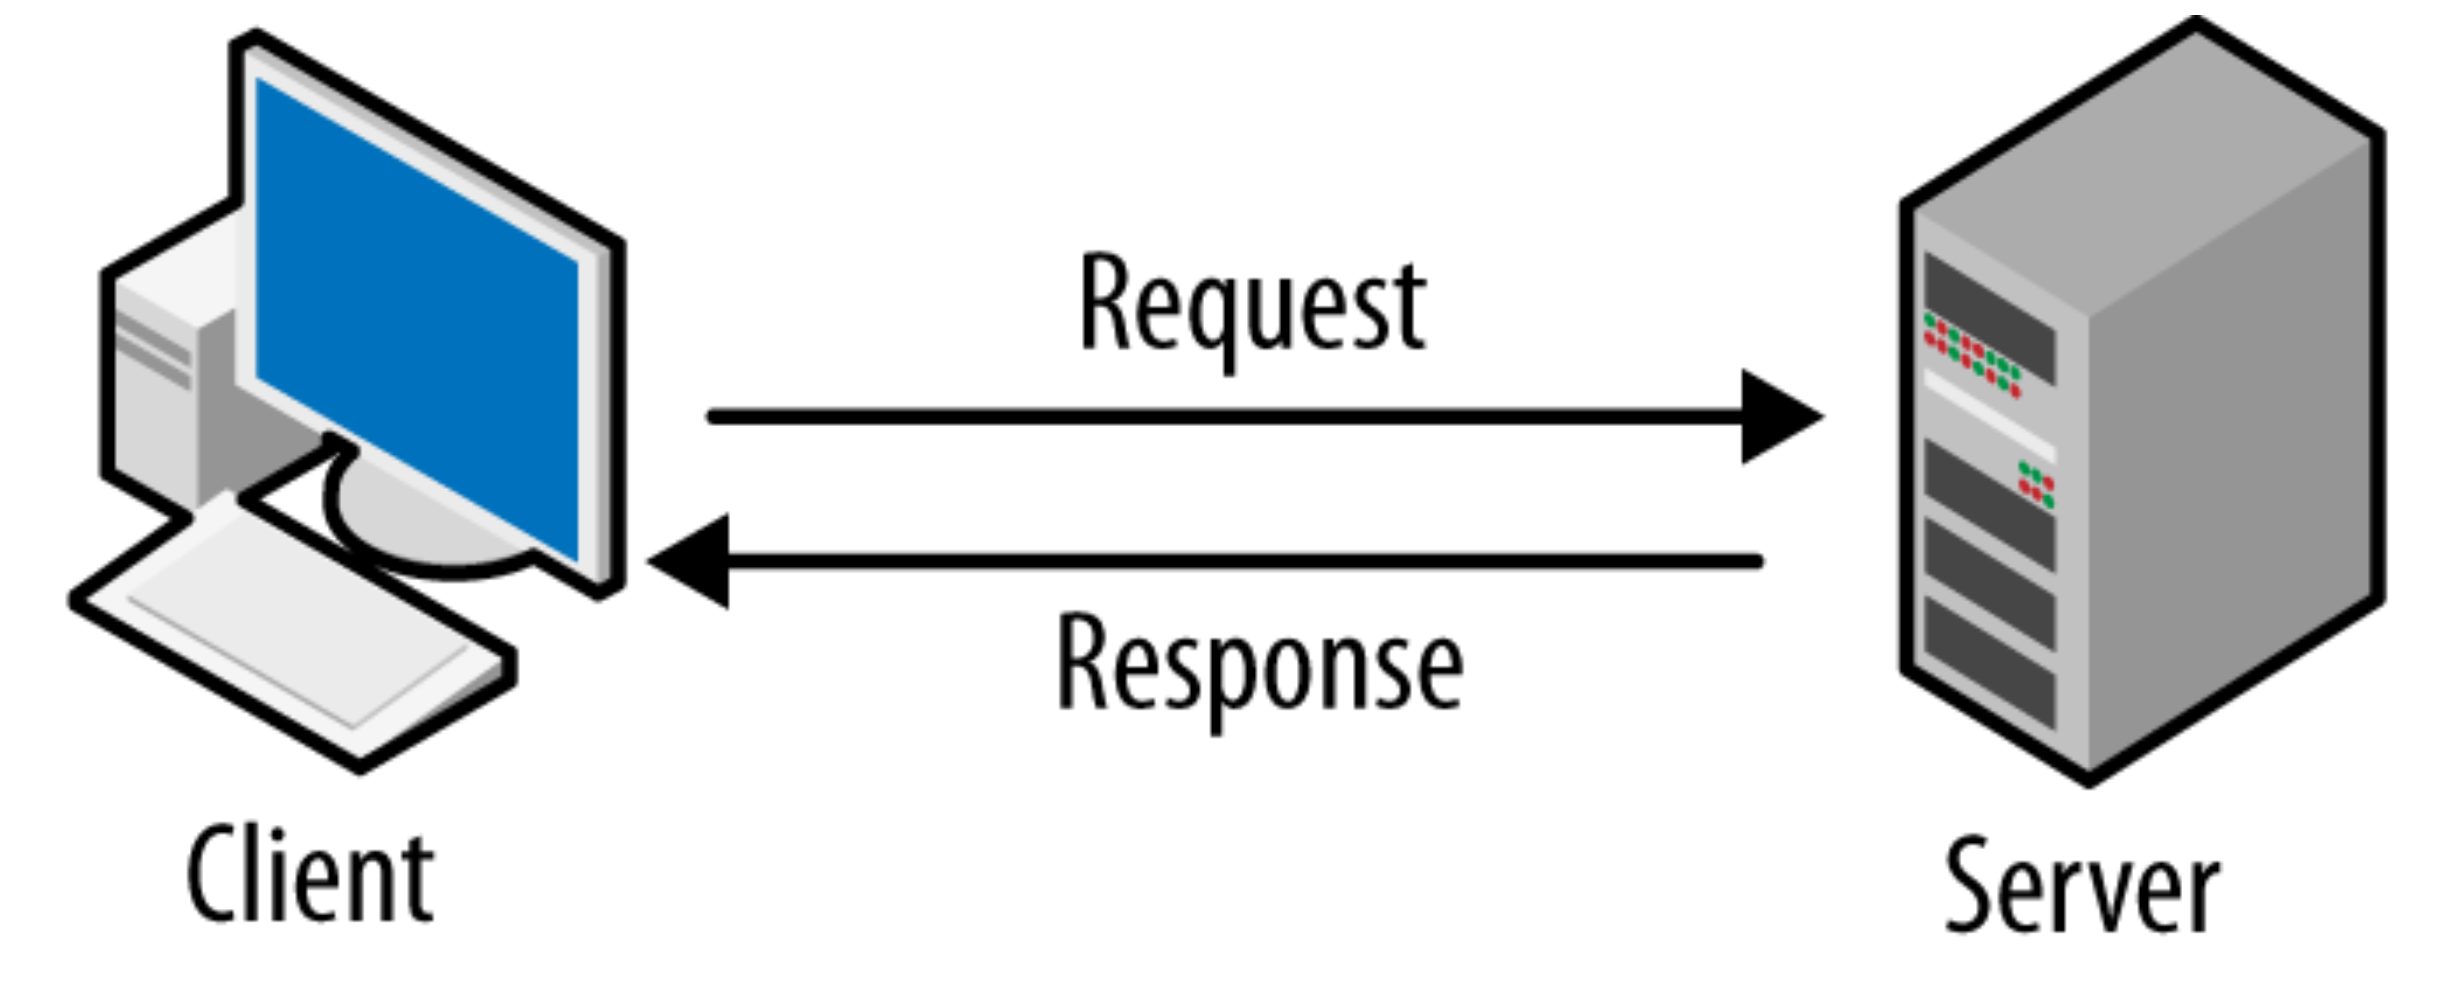
\includegraphics[width=0.8\linewidth]{figures/request_response.png}
	\caption{Request/Response Modell}
\end{figure}

\begin{table}[H]
	\begin{tabular}{c|c|c|c}
		URL: & https:// & www.google.com/ & index.html \\
		\hline
		& Protokoll & Domain IP-Adresse (DNS) & Ordnerstruktur, Datei
	\end{tabular}
\end{table}

\subsection*{Befehle}
Get, Post, Put, Delete,...

Bei HTTP ist alles im Klartext. \\
Bei HTTPS wird zusätzlich mit SSL/TLS verschlüsselt.

\subsection*{E-Mail}
\begin{table}[H]
	\begin{tabular}{c|c|c|c}
		E-Mail-Adresse: & name & @ & gmail.com \\
		\hline
		& Benutzername & & Domain
	\end{tabular}
\end{table}

\subsection*{SMTP (Port 25, TCP)}
Senden von Emails. Wird zum Senden von Mails und dem Weiterleiten zum Zielserver benutzt. SMTP kann zusätzlich Feedback geben (z.b. Ziel nicht erreichbar,...).

\subsection*{POP (Port 110, TCP)}
Empfangen von E-Mails. Man erhält vom Server das Original. Die Mail wird am Server gelöscht (Vorteil: Speicherplatz, Security).

\subsection*{IMAP (Port 143, TCP)}
Empfangen von E-Mails. Man erhält vom Server eine Kopie. Das Original bleibt am Server gespeichert (Vorteil: Verbindung mit mehreren Geräten ist praktisch, Backup).

	
	\chapter{template}
\section{image}

\begin{figure}[H]
	\centering
	
\includegraphics[width=0.8\linewidth]{figures/test.jpg}
	\caption{image example}
\end{figure}

\section{code}
Quellcode \ref{code:code_ex} 

\lstinputlisting[style=Java, label={code:code_ex}, caption={code include example}, captionpos=b]{code/code.java}
	
	
%-------------------------------------------------------------------------------------------%
% VERZEICHNISSE
	\pagenumbering{Roman}
	\setcounter{chapter}{0}
	\renewcommand{\thechapter}{\Roman{chapter}} 

	\listoffigures

	\listoftables	
	
	\lstlistoflistings
	
	\printbibliography

\end{document}